%%% The main file. It contains definitions of basic parameters and includes all other parts.

%% Settings for single-side (simplex) printing
% Margins: left 40mm, right 25mm, top and bottom 25mm
% (but beware, LaTeX adds 1in implicitly)
\documentclass[12pt,a4paper]{report}
\setlength\textwidth{145mm}
\setlength\textheight{247mm}
\setlength\oddsidemargin{15mm}
\setlength\evensidemargin{15mm}
\setlength\topmargin{0mm}
\setlength\headsep{0mm}
\setlength\headheight{0mm}
% \openright makes the following text appear on a right-hand page
\let\openright=\clearpage

%% Settings for two-sided (duplex) printing
% \documentclass[12pt,a4paper,twoside,openright]{report}
% \setlength\textwidth{145mm}
% \setlength\textheight{247mm}
% \setlength\oddsidemargin{14.2mm}
% \setlength\evensidemargin{0mm}
% \setlength\topmargin{0mm}
% \setlength\headsep{0mm}
% \setlength\headheight{0mm}
% \let\openright=\cleardoublepage

\usepackage{ulem}

%% Generate PDF/A-2u
\usepackage[a-2u]{pdfx}

%% Character encoding: usually latin2, cp1250 or utf8:
\usepackage[utf8]{inputenc}

%% Prefer Latin Modern fonts
\usepackage{lmodern}

%% Further useful packages (included in most LaTeX distributions)
\usepackage{amsmath}        % extensions for typesetting of math
\usepackage{amsfonts}       % math fonts
\usepackage{amsthm}         % theorems, definitions, etc.
\usepackage{bbding}         % various symbols (squares, asterisks, scissors, ...)
\usepackage{bm}             % boldface symbols (\bm)
\usepackage{graphicx}       % embedding of pictures
\usepackage{fancyvrb}       % improved verbatim environment
\usepackage{natbib}         % citation style AUTHOR (YEAR), or AUTHOR [NUMBER]
\usepackage[nottoc]{tocbibind} % makes sure that bibliography and the lists
			    % of figures/tables are included in the table
			    % of contents
\usepackage{dcolumn}        % improved alignment of table columns
\usepackage{booktabs}       % improved horizontal lines in tables
\usepackage{paralist}       % improved enumerate and itemize
\usepackage{xcolor}         % typesetting in color

\usepackage{todonotes}
\usepackage{subcaption}
\usepackage{moreverb}
\usepackage[T1]{fontenc}
\usepackage[acronym]{glossaries}
\usepackage{amsthm}

\theoremstyle{definition}
\newtheorem{definition}{Definition}[section]
\usepackage{mathtools, nccmath}

\DeclarePairedDelimiter{\nint}\lfloor\rceil
\DeclarePairedDelimiter\floor{\lfloor}{\rfloor}
\DeclarePairedDelimiter\ceil{\lceil}{\rceil}
\DeclarePairedDelimiter{\abs}\lvert\rvert
\makeglossaries

\newacronym{som}{SOM}{Self-organizing map}
\newacronym{bmu}{BMU}{Best Matching Unit}
\newacronym{pca}{PCA}{Principal Component Analysis}
\newacronym{rgb}{RGB}{Red Green Blue color model}
\newacronym{cbir}{CBIR}{Content-based image retrieval}
\newacronym{kis}{KIS}{Known-item search}
\newacronym{cnn}{CNN}{Convolutional Neural Network}
\newacronym{iou}{IoU}{Intersection over Union}
\newacronym{dnn}{DNN}{Deep Neural Network}
\newacronym{api}{API}{Application programming interface}
\newacronym{vbs}{VBS}{Video Browser Showdown}


%%% Basic information on the thesis

% Thesis title in English (exactly as in the formal assignment)
\def\ThesisTitle{Searching Image Collections Using Deep Representations of Local Regions}

% Author of the thesis
\def\ThesisAuthor{Jana Bátoryová}

% Year when the thesis is submitted
\def\YearSubmitted{2020}

% Name of the department or institute, where the work was officially assigned
% (according to the Organizational Structure of MFF UK in English,
% or a full name of a department outside MFF)
\def\Department{Department of Software Engineering}

% Is it a department (katedra), or an institute (ústav)?
\def\DeptType{Department}

% Thesis supervisor: name, surname and titles
\def\Supervisor{doc. RNDr. Jakub Lokoč, Ph.D.}

% Supervisor's department (again according to Organizational structure of MFF)
\def\SupervisorsDepartment{Department of Software Engineering}

% Study programme and specialization
\def\StudyProgramme{Computer Science}
\def\StudyBranch{Artificial Intelligence}

% An optional dedication: you can thank whomever you wish (your supervisor,
% consultant, a person who lent the software, etc.)
\def\Dedication{%
Firstly, I would like to thank my supervisor doc. RNDr. Jakub Lokoč, Ph.D. for ideas, numerous corrections, and spot-on help. My thanks also go to the SIRET Research group members for sharing their experience and knowledge in the research topic with me. Last but not least, I thank all the faculty members and especially fellow students. They created an amazing growth environment where I could learn. Personal thanks go to my close friends and family, who helped me persist in my studies.
}

% Abstract (recommended length around 80-200 words; this is not a copy of your thesis assignment!)
\def\Abstract{%
In a known-item search task (KIS), the goal is to find a previously seen image in a multimedia collection. In this thesis, we discuss two different approaches based on the visual description of the image.

In the first one, the user creates a collage of images (using images from an external search engine), based on which we provide the most similar results from the dataset. Our experiments show that we can provide more relevant results when incorporating spatial information by splitting the images into several parts. We compared this approach to a baseline, which does not utilize this spatial information and an approach that alters a layer in a deep neural network.

We also present an alternative approach to the KIS task, search by faces. In this approach, we work with the faces extracted from the images. We investigate face representations for their ability to sort people based on their similarity. Based on these similarities, we build a structure that allows easy exploration of the set of faces.

We provide a demo, implementing all presented techniques.
}

% 3 to 5 keywords (recommended), each enclosed in curly braces
\def\Keywords{%
{Known-Item-Search} {Convolutional Neural Network} {Content-based image retrieval} {Multimedia exploration}
}

%% The hyperref package for clickable links in PDF and also for storing
%% metadata to PDF (including the table of contents).
%% Most settings are pre-set by the pdfx package.
\hypersetup{unicode}
\hypersetup{breaklinks=true}

% Definitions of macros (see description inside)
%%% This file contains definitions of various useful macros and environments %%%
%%% Please add more macros here instead of cluttering other files with them. %%%

%%% Minor tweaks of style

% These macros employ a little dirty trick to convince LaTeX to typeset
% chapter headings sanely, without lots of empty space above them.
% Feel free to ignore.
\makeatletter
\def\@makechapterhead#1{
  {\parindent \z@ \raggedright \normalfont
   \Huge\bfseries \thechapter. #1
   \par\nobreak
   \vskip 20\p@
}}
\def\@makeschapterhead#1{
  {\parindent \z@ \raggedright \normalfont
   \Huge\bfseries #1
   \par\nobreak
   \vskip 20\p@
}}
\makeatother

% This macro defines a chapter, which is not numbered, but is included
% in the table of contents.
\def\chapwithtoc#1{
\chapter*{#1}
\addcontentsline{toc}{chapter}{#1}
}

% Draw black "slugs" whenever a line overflows, so that we can spot it easily.
\overfullrule=1mm

%%% Macros for definitions, theorems, claims, examples, ... (requires amsthm package)

\theoremstyle{plain}
\newtheorem{thm}{Theorem}
\newtheorem{lemma}[thm]{Lemma}
\newtheorem{claim}[thm]{Claim}

\theoremstyle{plain}
\newtheorem{defn}{Definition}

\theoremstyle{remark}
\newtheorem*{cor}{Corollary}
\newtheorem*{rem}{Remark}
\newtheorem*{example}{Example}

%%% An environment for proofs

\newenvironment{myproof}{
  \par\medskip\noindent
  \textit{Proof}.
}{
\newline
\rightline{$\qedsymbol$}
}

%%% An environment for typesetting of program code and input/output
%%% of programs. (Requires the fancyvrb package -- fancy verbatim.)

\DefineVerbatimEnvironment{code}{Verbatim}{fontsize=\small, frame=single}

%%% The field of all real and natural numbers
\newcommand{\R}{\mathbb{R}}
\newcommand{\N}{\mathbb{N}}

%%% Useful operators for statistics and probability
\DeclareMathOperator{\pr}{\textsf{P}}
\DeclareMathOperator{\E}{\textsf{E}\,}
\DeclareMathOperator{\var}{\textrm{var}}
\DeclareMathOperator{\sd}{\textrm{sd}}

%%% Transposition of a vector/matrix
\newcommand{\T}[1]{#1^\top}

%%% Various math goodies
\newcommand{\goto}{\rightarrow}
\newcommand{\gotop}{\stackrel{P}{\longrightarrow}}
\newcommand{\maon}[1]{o(n^{#1})}
% \newcommand{\abs}[1]{\left|{#1}\right|}
\newcommand{\dint}{\int_0^\tau\!\!\int_0^\tau}
\newcommand{\isqr}[1]{\frac{1}{\sqrt{#1}}}

%%% Various table goodies
\newcommand{\pulrad}[1]{\raisebox{1.5ex}[0pt]{#1}}
\newcommand{\mc}[1]{\multicolumn{1}{c}{#1}}


% Title page and various mandatory informational pages
\begin{document}
%%% Title page of the thesis and other mandatory pages

%%% SPECIMEN
%%% Inscriptions at the opening page of the hard cover

\pagestyle{empty}
\hypersetup{pageanchor=false}
\XXX{Opening page of the hard cover. Not a part of the electronic version.}
\begin{center}

\large
Charles University

\medskip

Faculty of Mathematics and Physics

\vfill

{\huge\bf BACHELOR THESIS}

\vfill

\hbox to \hsize{\YearSubmitted\hfil \ThesisAuthor}

\end{center}

\newpage\openright

%%% NEMICEPS

%%% Title page of the thesis

\pagestyle{empty}
\hypersetup{pageanchor=false}
\begin{center}

\centerline{\mbox{
\includegraphics[width=166mm]{img/logo-en.pdf}}}

\vspace{-8mm}
\vfill

{\bf\Large BACHELOR THESIS}

\vfill

{\LARGE\ThesisAuthor}

\vspace{15mm}

{\LARGE\bfseries\ThesisTitle}

\vfill

\Department

\vfill

{
\centerline{\vbox{\halign{\hbox to 0.45\hsize{\hfil #}&\hskip 0.5em\parbox[t]{0.45\hsize}{\raggedright #}\cr
Supervisor of the bachelor thesis:&\Supervisor \cr
\noalign{\vspace{2mm}}
Study programme:&\StudyProgramme \cr
\noalign{\vspace{2mm}}
Study branch:&\StudyBranch \cr
}}}}

\vfill

% Zde doplňte rok
Prague \YearSubmitted

\end{center}

\newpage

%%% NOPHD
%%% Here should be a bound sheet included -- a signed copy of the "bachelor
%%% thesis assignment". This assignment is NOT a part of the electronic
%%% version of the thesis. DO NOT SCAN.
\XXX{Bound into the introductory part must be the form with signed approval of the thesis topic (a photocopy suffices).
This is not a~part of the electronic version of the thesis, do not scan!}
%%% PHDNO

%%% A page with a solemn declaration to the bachelor thesis

\openright
\hypersetup{pageanchor=true}
\pagestyle{plain}
\pagenumbering{roman}
\vglue 0pt plus 1fill

\noindent
I declare that I carried out this bachelor thesis independently, and only with the cited
sources, literature and other professional sources. It has not been used to obtain another
or the same degree.

\medskip\noindent
I understand that my work relates to the rights and obligations under the Act No.~121/2000 Sb.,
the Copyright Act, as amended, in particular the fact that the Charles
University has the right to conclude a license agreement on the use of this
work as a school work pursuant to Section 60 subsection 1 of the Copyright~Act.

\vspace{10mm}

\hbox{\hbox to 0.5\hsize{%
In \hbox to 6em{\dotfill} date \hbox to 6em{\dotfill}
\hss}\hbox to 0.5\hsize{\dotfill\quad}}
\smallskip
\hbox{\hbox to 0.5\hsize{}\hbox to 0.5\hsize{\hfil Author's signature\hfil}}

\vspace{20mm}
\newpage

%%% Dedication

\openright

\noindent
\Dedication

\newpage

%%% Mandatory information page of the thesis

\openright

\vbox to 0.5\vsize{
\setlength\parindent{0mm}
\setlength\parskip{5mm}

Title:
\ThesisTitle

Author:
\ThesisAuthor

\DeptType:
\Department

Supervisor:
\Supervisor, \SupervisorsDepartment

Abstract:
\Abstract

Keywords:
\Keywords

\XXX{This information must be stored as PDF meta-data, too. Please refer to the {\tt README} file.}
\vss}

\newpage

\openright
\pagestyle{plain}
\pagenumbering{arabic}
\setcounter{page}{1}


%%% A page with automatically generated table of contents of the master thesis

\tableofcontents

%%% Each chapter is kept in a separate file
\chapter*{Introduction}
\addcontentsline{toc}{chapter}{Introduction}

In the last decades, we have witnessed a massive jump in the amount of digital information owned by individuals. Looking back 20-30 years, people used to record only a few hours of their lives, capturing precious moments. Now, according to available estimates, more than 500 hours of videos is uploaded every minute  to YouTube\footnote{\href{https://www.statista.com/statistics/259477/hours-of-video-uploaded-to-youtube-every-minute/}{Statista -- Hours of video uploaded to YouTube every minute}} only. Furthermore, decreasing prices and increasing availability of the recording electronics (especially smartphones) contribute to the amount of multimedia data created every day. It has also become a trend to share videos from day-to-day lives.

The significant increase in the volume of multimedia data opens several new challenges. One of the most vital is the need for effective search and retrieval. This problem is not only attractive to researchers, but the initiative also comes from the industry. Companies try to help their customers to organize a vast amount of multimedia data (Google Photos, Facebook, OneDrive, MEGA, and others). Those companies often rely on a broad spectrum of techniques used to store and organize the data internally. Unfortunately, users are usually provided with only the most straightforward technique to filter the data.

Besides attempting to overcome the challenges of querying large volumes of stored data, we will focus on a challenging scenario in which a user searches for one given image in a dataset. This task of searching for a previously seen multimedia object is often referred to as visual known-item search (\acrshort{kis}). In this thesis, we investigate several known-item search techniques where users provide a few example images as a collage query or browse through images of faces organized in a grid with respect to their similarity.

Known-item search has become a well-known research area \citep{8352047}. According to recent findings \citep{9037125}, most of the known-item search engines incorporate both querying and interactive search functionality. In order to elevate the level of developed KIS systems, researchers organize and participate in annual competitions. These efforts help to increase the interest in user-centered multimedia search. One, for example, is Video Browser Showdown\footnote{\url{https://videobrowsershowdown.org/}}, or shortly VBS. For a comparison, TRECVid \citep{2019trecvidawad} is also an annual competition with the main focus on ranking of scenes based on a textual description.

In this thesis, we investigate a couple of approaches to solve the known-item search task:

\begin{enumerate}
  \item Searching by an image collage query.
  \item Searching by browsing in a set of faces from the dataset.
\end{enumerate}

In the first approach, we focus on searching known images via only example images and their approximate position in the searched image. Users can create a collage of images that reminds them of the searched scene and then browse through the ranked result list looking for the match.

The second approach is an experimental test of the possibility of visual traversing through a dataset of faces. To present a user with a feasible amount of faces in one display, we tackle this challenge by organizing the faces into multilevel view supporting navigational queries. We implemented the traversal system, although we found out that this technique is less effective than other retrieval techniques presented in this thesis.

The goal of this thesis is to create a framework to test both approaches, as mentioned earlier. We aim to create a novice-friendly interface for smooth user-system interaction.

For the techniques which searching by the collages, We provide evaluations on an annotated set of queries. We manually created a set of collages, as our queries. We use them to test different hyperparameters of the proposed system. We evaluate the proposed methods based on the rank of the target image. Well-performing methods bring the searched items to the foreground, placing them at the top ranks.

We evaluate the second approach -- search based on faces -- with the help of a case study. We firstly investigate the space of the feature vectors by evaluating the responses from the survey. Then we present the solution. In the end, we provide a comparison between the average time needed to find a target face. We compare our traversal system to a display of randomly ordered faces.

\subsubsection*{Thesis structure}
The thesis is divided into four main chapters. After the Introduction, we continue by reviewing Related Work (\autoref{ch:related_work}) and Content-based image retrieval (\autoref{ch:preliminaries}). Related Work previews several existing frameworks for solving the KIS task. Content-based image retrieval chapter contains some elementary theoretical background for CBIR tasks and also evaluation settings.

After these introductory chapters, we present investigated approaches in chapters \ref{ch:object_location} and \ref{ch:face_search}. \todo{ref}

The end of the thesis is dedicated to the implementation of the aforementioned approaches. This includes the user's guide -- how to interact with the system, and developer's guide -- how to modify the dataset or how to incorporate a new approaches.

\bigskip

In summary, we designed and successfully tested a promising approach based on collage queries. The most promising approach splits images into multiple parts. We also developed a traversal system for previewing a dataset of faces. The experiments show, that using it decreased time of the individual search by XX\% \todo{}.
\chapter{Related work}
\label{ch:related_work}


This chapter reviews approaches made towards handling Known-item Search (KIS) task and the recent approaches for user-friendly traverse through the immersive amount of the visual data.

In recent years, we witnessed a significant advancement in the solution for the KIS task. The scale of the solution's complexity for user interaction ranges from simple ones (e.g., sketching color blocks) with only a few descriptors to the ones which use recent advance in deep learning, as for concept labeling (i.e, naming objects).

Our goal is to perform known-item-search task on a set of videos. We perform a common simplification, replacing videos with the set of images. We do this, since we look for a particular scene, which can be also an image. This level of abstraction therefore corresponds to the searched query. Also, this allows us to use a potential of a common neural networks and other solutions presented for 2D data (images in our case). For this task we perform sampling over the videos. More information is available in section \ref{}\todo{fix}, where more details about the dataset are available.

\section*{Known-item-search Task}

Known-item-search task is present in many different situations. The tasks is to efficiently retrieve a known item in the dataset. For example, for a database of newspaper article we may use such retrieval tools to find a particular article we are interested in. Our thesis focuses on visual KIS task, specifically we retrieve images. For the setting we solve our task in exist even annual competitions to share the knowledge and the advancements. One of such is Video Browser Showdown \ref{}\todo{fix}, which is taking place since 2012. We review a few of the presented solutions to this task from the last VBS2019. We mainly follow the summarization in the \ref{}\todo{fix}

The most common approach at the VBS2019 were "Query by an Image" and "Concept Labeling". Query by an image, in this case, mostly refers to finding the most similar results from databse to given image. The downside of this approach is mainly the difficulty to obtain an image, which would be sufficiently similar to the searched one.

The second most used approach at VBS2019 was Concept Labelling. In this case, a user can describe the scene using the words. The database is pre-annotated with the vocabulary of present items. During the request, the algorithm checks the database for the presence of the searched concept. This approach has a limitation of the vocabulary size. Recent advancement in the textual annotation neural networks is nowadays able to describe thousands of different objects by words, but still, this may present on the limitation on rarely used objects or hard to describe objects.

One of the approaches presented and used is by creating a color sketch. The user colors the canvas with respect to the original searched scene. The database is then traversed on the correspondence of the colors to the particular part of the image. We see a significant advantage of this approach to distinguish between the key objects in the scene spatially.
 
Solving KIS task in VBS setting offers the option of using full video information and not only snapshots. This approach enhances the possibilities spectrum to Temporal Queries or Multimodal queries. Also, the solution included Optical Character Recognition (OCR) was presented. We present our solution as a possible enhancement of a complex system in order to create multiple search strategies based on user-preference. 

\section*{Traversion Approaches}

Since the KIS task is the task of two sides -- the algorithm and the user, it is essential to not forget about the easy to use interface. A good overview of the dataset may hide some deficiencies of the algorithm so that the user can still find the search scene. As the  (Evaluation of VBS ref)\todo{fix} shows, the most common approach is to show a 2D grid of images to the user. Several approaches also provide an easy way to play the original video as one of the most immersive ways we have encountered to traverse a grid of images is placing these images on the globe with the possibility of multiway traversing (TODO: ref). We aim to achieve a similar level of smooth traversing.

The traversing systems rely on effective visualization techniques on high-number feature spaces. These systems create mostly a 2D grid of the images based on the distance between the samples in high dimensionality space. Though, this high dimensionality space, often produced by neural networks, may not have feasible representation in 2D space based on the hidden features. This is often caused by a lack of understanding and representability of the deep features. We aim to test this feature reduction to the 2D test in our face experiment with the use of deep neural network features.

\section{Existing systems}

In the next section we shortly investigate on existing frameworks, which competed in the Video Browser Showdown.

\subsection{VIRET}

A framework named VIRET (\cite{lokovc2019framework, lokovc2019viret}) is successfully participating in the competitions for a several years now. The framework evolved in the years and now it offers a wide variety of the strategies for solving KIS task. VIRET also implements own strategy for a frame selection, which we also used for obtaining our images. As one of the biggest strategical advantages of the VIRET we consider a multi-modal queries with relevance scores and update of the queries based on the results. We take VIRET as our inspiration and we do not implement the same approaches as are already present in the VIRET. We focus on testing new alternatives.

\begin{figure}
    \centering
    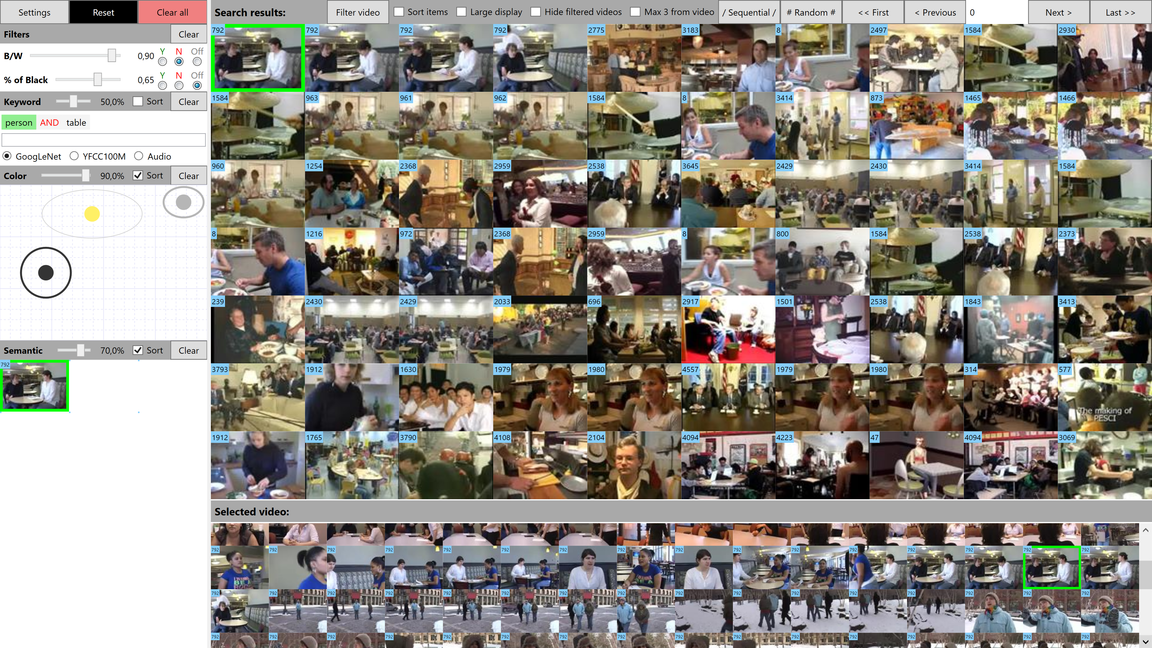
\includegraphics{img/viret_small.png}
    \caption{A sample search in VIRET framework. Source: https://videobrowsershowdown.org/hall-of-fame/}
    \label{fig:viret}
\end{figure}

\subsection{SOM Hunter}

A SOM Hunter (\cite{kratochvil2020som}) was for the first time introduced at the VBS2020. This tool is related to us, since it successfully proved using Self-organizing Maps for a use in a Known-item-search task. They train a small self-organizing map on the fly over only a sample of the dataset. This allows them to recreate the SOM based on the user interaction and train it on the fly. In our work we use the idea of training SOM, but compared to the SOM Hunter we will test creating a SOM only on the faces of the people.

\begin{figure}
    \centering
    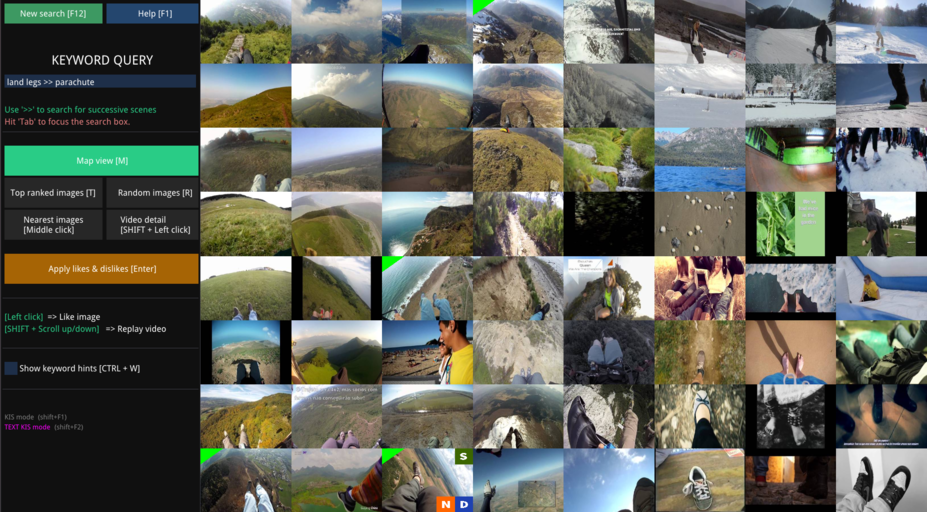
\includegraphics[width=0.99\linewidth]{img/som_hunter_small.png}
    \caption{A sample search in SOM Hunter. Source: https://videobrowsershowdown.org/hall-of-fame/}
    \label{fig:som_hunter}
\end{figure}

\subsection{Vitrivr}

Vitrivr (\cite{rossetto2016vitrivr}) is one part of more complex solution for retrieving a video in the collection. Vitrivr is the module responsive for creating queries which are then processed by the Cineast. The overview of the system is displayed in the figure \ref{fig:vitrivr}. The Vitrivr supports different query types, as query by a sketch, example image, semantic concept, keywords, audio or motion. The feature extraction and the system behind retriving the most similar results are part of the second module -- Cineast (\cite{rossetto2016searching}). Cineast uses multiple approaches incorporating deep features, i.e. scene text recognition and speech-to-text recognition. The Vitrivr (part responsible for creating the queries) is a web-browser solution, therefore the tool includes a clean separation between the query formulation and retrieving the responses.

\begin{figure}
    \centering
    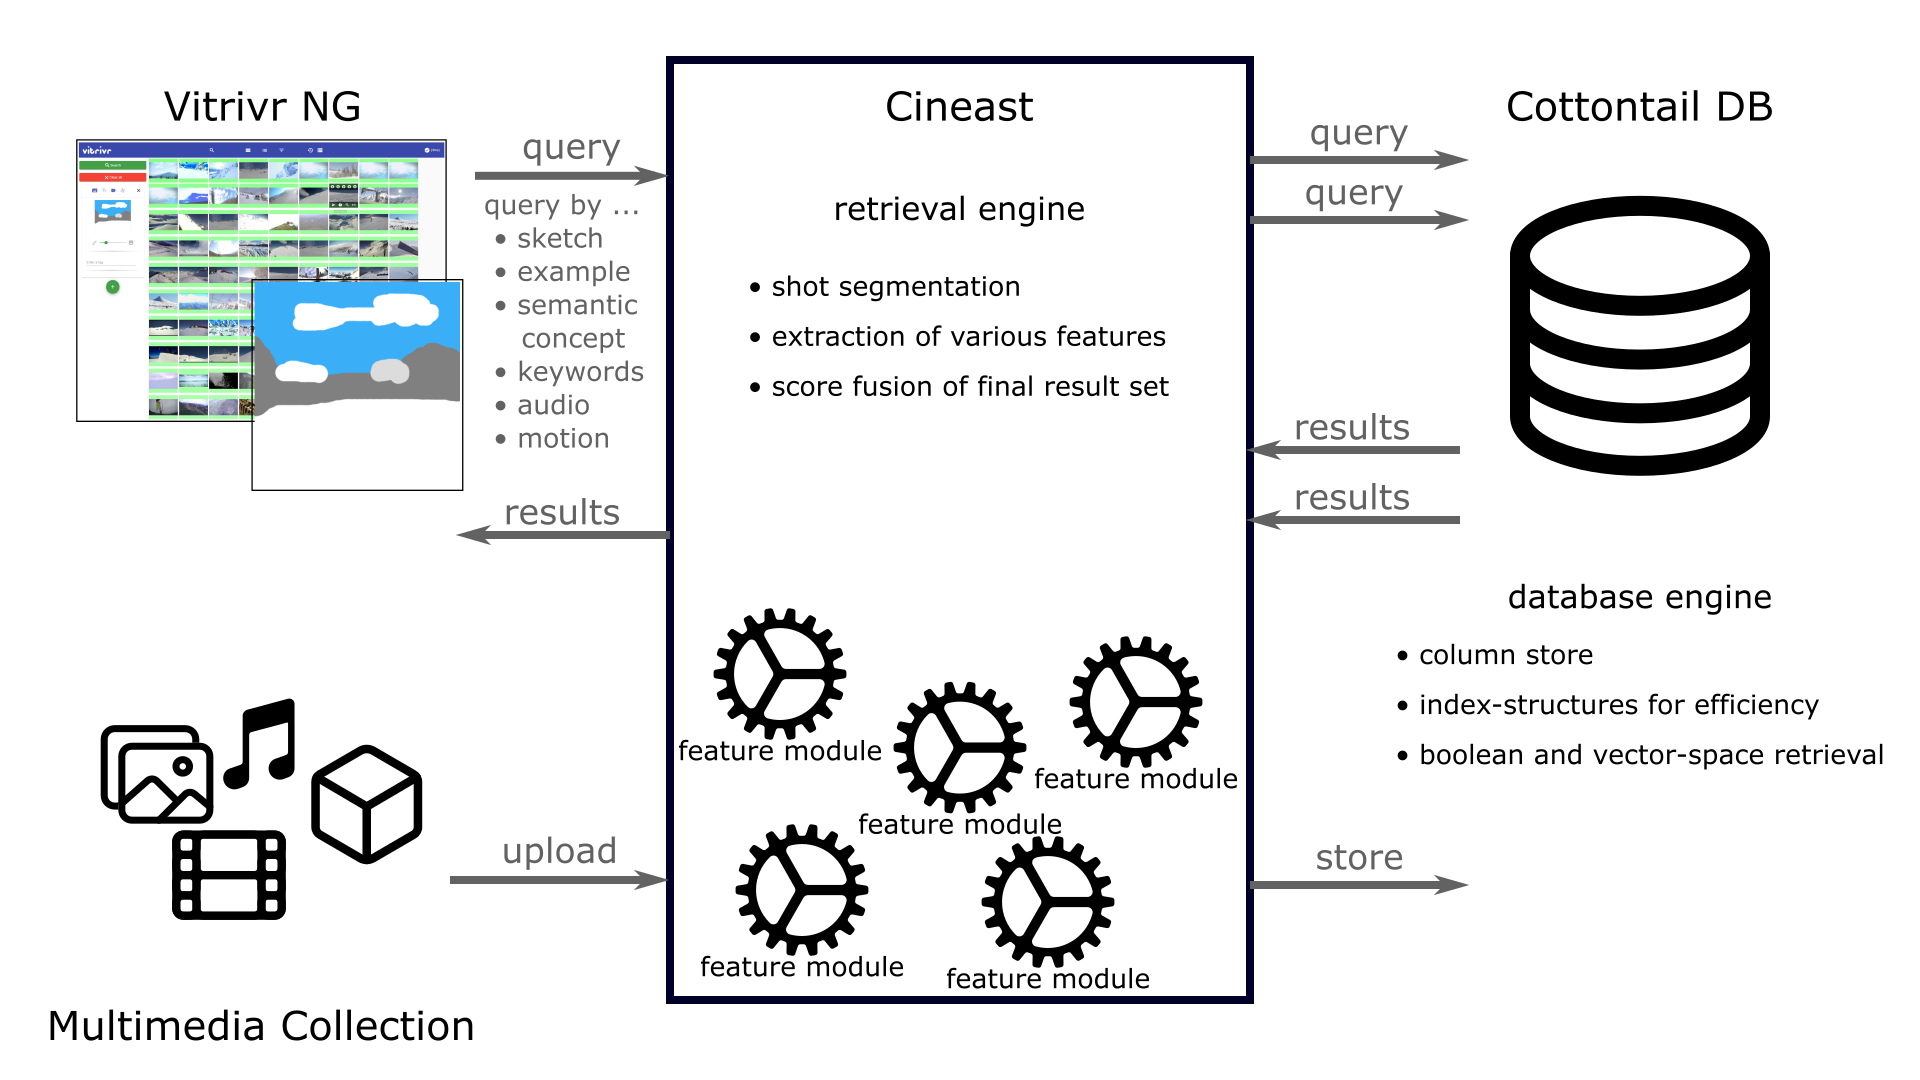
\includegraphics[width=\linewidth]{img/vitrivr.png}
    \caption{Overview of the separation in the Vitrivr solution. Source: \url{https://vitrivr.org/vitrivr.html}}
    \label{fig:vitrivr}
\end{figure}

\section{Deep Neural Networks}

In recent years we witnessed many records-breaking new machine learning models. Many of those were possible, thanks to the advancement of Deep Neural Networks (DNN). Nowadays, these models replaced more traditional Machine Learning approaches in many tasks.

Deep Neural Network is a machine learning model, whose goal is to approximate a given function \(f\). The set of parameters is often referred to as \(\theta\). One of the everyday tasks performed by these networks is classification, where the goal of the network is to predict which category sample \(X\) belongs. Even though we will not perform a classification task in this thesis, we will use some of the available classification networks.

When we talk about neural networks, we usually refer to a feedforward network. These networks consist of layers where information during the evaluation is passed only in one direction. We can imagine it as applying a function to the results from the previous layer. For example, let us create a small neural network. Denote first layer as \(f_1\) and second layer as \(f_2\). The output of the network will be \(f_2\left(f_1\left(\right)\right)\).

Stacking more and more layers on top of each other leads us to notation \emph{deep} neural networks. This notation has no fixed threshold on which networks "deserve" to be called deep. Therefore we do not recognize any importance to the naming "deep." 

The first and last layer are commonly referenced as \emph{input} and \emph{output} layer. Layers between the input and output layers are usually denoted as \emph{hidden} layers. Deep neural networks can have four or hundreds of layers, and each layer of the layer can have even a unique structure. \emph{Network Architecture} captures the "build order" of the network. It is important to note that there exist many networks with different architectures solving the same task.

There are many reasons for the advancement of neural networks in the past years. One of the crucial stones was not only theoretical innovations used for the networks but increasing computability limits. Deep Neural Networks \emph{learn} to approximate function by \emph{training}. This training is usually the heaviest part of the computation. Even though it is enough to train once and use forever, it usually lays some limitations on the size of the networks or the functions used.

Since this topic is broad, we recommend more thorough reading, such as Neural Networks and Deep learning online book\footnote{http://neuralnetworksanddeeplearning.com/}.

\subsection{Convolution Neural Networks}

Convolution Neural Networks (CNN) are a class of Deep Neural Networks. Even though they emerged in the late 1980s (\cite{lecun1989backpropagation}), it took another 20 years for further advancements in the research area. Convolution Neural Networks are mainly used in image-related tasks, such as image classification ("What is on the image?"), object detection ("Where are the objects in the image and what are they?") or even content generation ("Create a new image"). Their abilities were also tested in many, not image-related tasks, e.g., music genre recognition.

Convolution Neural Networks are specialized kind of networks which work with grid-like topology. For 1D can be an example as time-series, or for 2D, most typically image pixels represent a grid. The name \emph{convolution} refers to using a mathematical linear function \emph{convolution} in at least the layers. A simplified overview of the structure is displayed in figure \ref{fig:convolution_neural_network}. We refer to \cite{Goodfellow-et-al-2016} for more understanding of \emph{convolutional layers}.

\begin{figure}
    \centering
    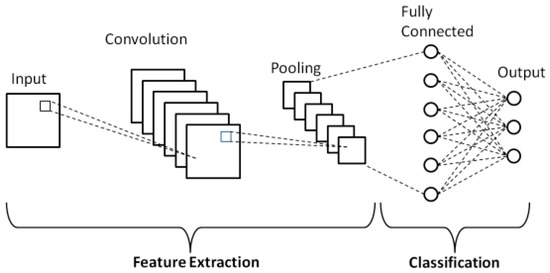
\includegraphics[width=0.98\textwidth]{img/convolution_neural_network.jpg}
    \caption{Schematic diagram of a basic convolution neural networks. Source: Phung, V.H.; Rhee, E.J. A High-Accuracy Model Average Ensemble of Convolutional Neural Networks for Classification of Cloud Image Patches on Small Datasets. Appl. Sci. 2019, 9, 4500.}
    \label{fig:convolution_neural_network}
\end{figure}

\subsection{Transfer Learning}

Transfer Learning is a research problem in machine learning that focuses on storing knowledge gained while solving one problem and applying it to a different problem. We have seen many successful transfers of the network architecture and parameters learned to a new task. Transfer learning helps to reduce the cost of the training and often also to overcome an insufficient set of training examples for the new task.

We utilize some of the pre-trained Convolution Neural Networks. The ability of a convolutional neural network to transfer to a new task by elevating gained information from other datasets was explored as early as by \cite{donahuedeep}, and many others were able to use this information to gain better models.  Networks we use are mostly pre-trained on \emph{ImageNet}\footnote{http://www.image-net.org/}. ImageNet served as a benchmark for comparing the performance of the different networks. Since the ImageNet is the main classification task, we utilize the transfer learning in a way to obtain deep features. Layers to the end of the networks accumulate more information, i.e., they contain high-level features. Therefore, we work with the layers close to the end of the networks. These layers represent encoded information about the image in high dimensional vectors. Our task is to use these deep features obtained for solving our known-search item task.


\begin{figure}
    \centering
	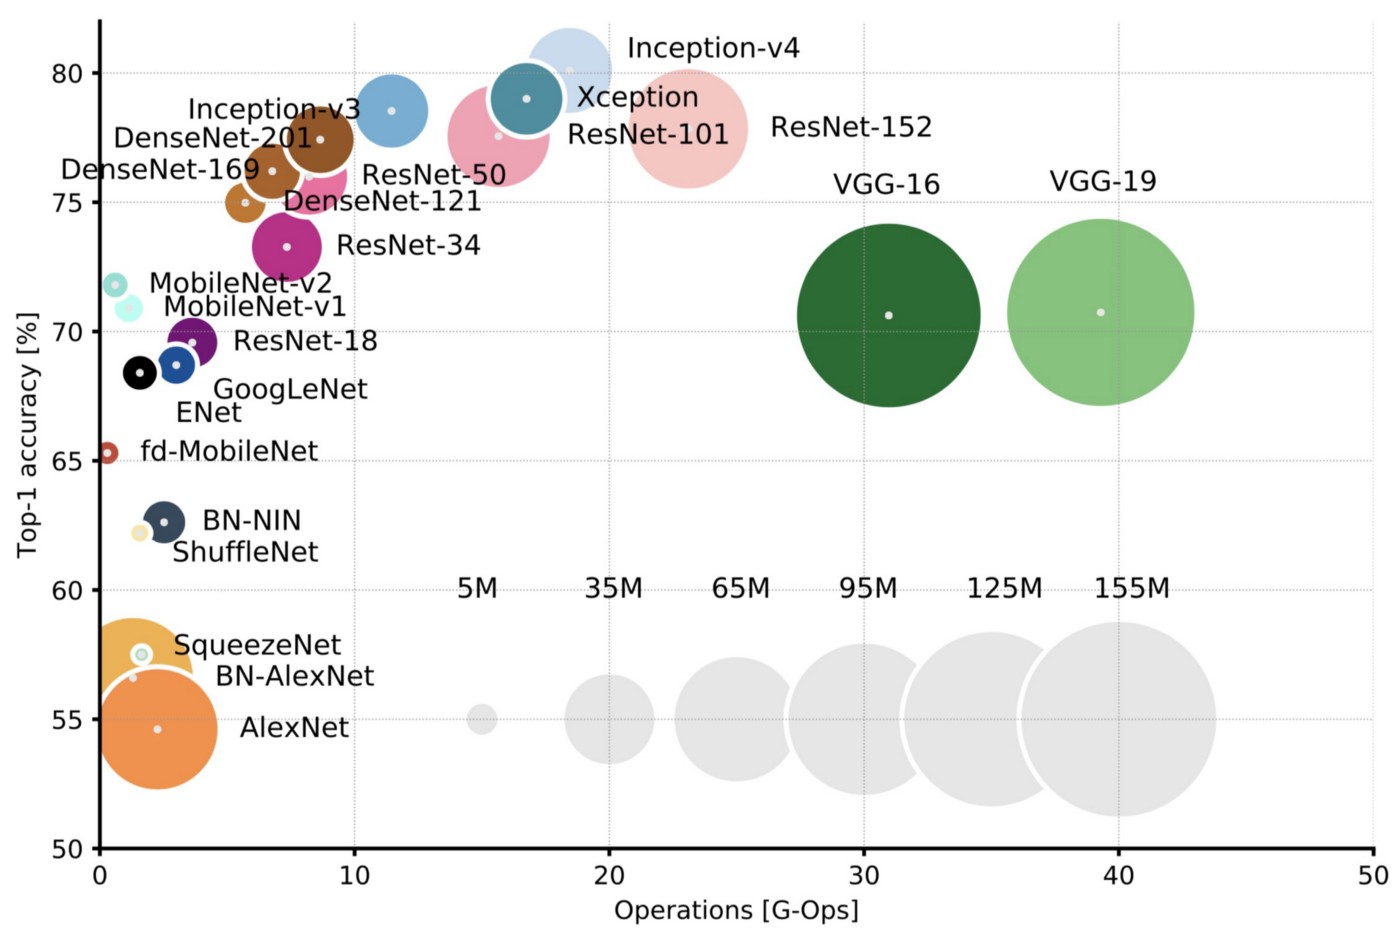
\includegraphics[width=0.8\linewidth]{img/network-comparison.jpeg}
	\caption{Top-1 one-crop accuracy versus amount of operations required for a single forward pass. The size of the blobs is proportional to the number of network parameters. Source: \cite{canziani2016analysis}}
	\label{fig:camera-setup}
\end{figure}

\subsection{Pretrained models}
\label{ss:pretrained_models}

\subsubsection{Keras}

Keras (\cite{chollet2015keras}) is a deep learning API written in Python, running on top of the machine learning platform TensorFlow\cite{tensorflow2015-whitepaper}. It was developed with a focus on experimentation in deep learning. We use it and its pre-trained models in this thesis. The models available in Keras Applications, which we use, were trained on ImageNet. Keras API allows us to separate the model from the last fully connected layer used for classification (since default ImageNet is a classification task). 

\subsection{Models Used}

\subsubsection*{Resnet50V2}
\cite{resnetv2} \cite{resnet}

\subsubsection*{MobileNetV2}
\cite{mobilenet} \cite{mobilenetv2}

\subsubsection{Dlib}
Dlib (\cite{king2009dlib}) is a modern C++ toolkit containing machine learning algorithms and tools for creating complex software in C++ to solve real-world problems. Some of the modules are provided with Python API. We use the Dlib library for face detection and also face feature extraction. For both we use face\_recognition API (\cite{geitgey2016machine}). \cite{king2017high} \todo{fix ref}





\chapter{Content-based Image Retrieval}
\label{ch:preliminaries}

Image retrieval and image indexing have been an active research field since the 1970s. In 1978 (\cite{tamura1978textural}), a group of researchers proposed a system for retrieving textures based on the example texture. Since then, a wide range of techniques for image retrieval were presented. Traditional approaches included manual annotation of the images by textual or numerical metadata. The user could then formulate a query against these annotations to retrieve relevant images. This approach is often referred to as Concept-based image retrieval or meta-data search.

There are several drawbacks to the textual or numerical annotations. First of all, extensive human annotations are often needed to provide rich data for filtering. Also, including spatial information of the objects takes more resources than only writing down present objects in the image. Furthermore, the images often include too many details (i.e., type, color, or shape of the objects), which may be impossible to comprehend by manual annotations.  The annotations may not even represent a stable truth. With a different annotator, the annotations may include different details/objects, which were perceived differently. When the user searches for an image, she has to know the exact terms the annotators used in order to be able to retrieve the images they want. As the last problem, we pose with human annotations is the scalability. As the amount of information increases every second, there is no human capability to hand process all the examples.

During the 1990s, content-based image retrieval (\acrshort{cbir}) emerged (trend study from \cite{datta2008image}). In the CBIR approach, the images are indexed by features directly derived from their visual content using automatic or semi-automatic image processing techniques. Such indexing lacks building blocks (for example, verbal description); on the other hand, it provides low-level feature information about the whole images or its regions. The attributes of images are complex functions of regions of the image or the whole image.

CBIR has received considerable research interest in the last decades. With the advancement in Deep Learning, a new pool of possible complex functions to describe the images emerged. In our approaches, we use pre-trained neural networks to extract features. Based on these features, we implemented and evaluated several approaches to the CBIR task.

Presented techniques focus on the known-item search task. An alternative could be an Ad Hoc search, where the goal is to retrieve all relevant items to the query. Known-item search task instead works with retrieving a known item from the dataset.

In the following chapters, we continue with the specifics of the individual approaches we present. Here we formulate the task and the goal.


\section{Task formulation}
\label{s:task_formulation_preliminaries}

The goal of the thesis is to propose a system that can search and retrieve images based on visual similarity.  

First we define universe $\mathcal{U}$ as the set of the all possible images:

$$
    \mathcal{U} = \bigcup_{h,w \in \mathbb{N}^2} \{0, 1, 2, \ldots, 255 \}^{h \times w \times 3}
$$

This definition follows the standard description of an image as a matrix $w \times h$ of pixels, where three color channels describe each pixel. We work over a dataset $D$ of such images, that we can define as $D \subset \mathcal{U}$.

% The user is then presented with a target image $t \in D$ and asked to locate the image within the dataset $D$. This task is called known-item search {\color{red} to je spis simulace toho tasku, ve skutecnosti si uzivatel obrazek T jen matne vzpomina}. 

The user is then asked to find a target image $t \in D$, that they have some knowledge of, for example, by (imperfectly) remembering the image or other detailed description. This task is called a known-item search.

Our system then serves as a search engine, aiming to provide the user with the most relevant results based on the user input. The system leverages the visual similarity between the images in the dataset $D$ (as in chapter \ref{ch:face_search}), or the similarity between user-provided example pictures and the images from the dataset $D$ (as in chapter \ref{ch:object_location}).

\section{Feature space}

To search over a dataset of images $D$, we need a metric of how similar two items are. This similarity could be computed between the images directly, although it is more common to compare their descriptors (i.e., their  projections by a descriptor extraction function). A descriptor extraction function is a function $f_e: \mathcal{U} \rightarrow \mathcal{F}$, where $\mathcal{F}$ is a feature space. Given a descriptor extraction function $f_e$, we compute for each image in the dataset $D$ a descriptor (or feature vector) $L_I = f_e(I)$, where $I \in \mathcal{U}, L_I \in \mathcal{F}$. In our work, we use various neural networks as our descriptor extraction functions. It is common for neural networks to produce the descriptors in the space of real numbers $\mathbb{R}^n$, and in our case, we work only with the descriptor spaces, which are isomorph to the $\mathbb{R}^n$.

\section{Distance Measures}
\label{s:distance_measures}

To compare, how similar descriptors of two images are, we use a concept of distance. Similar descriptors have smaller distance, and vice versa. We use a definitions for a distance space and metric space from the book \cite{deza2009encyclopedia}.

\theoremstyle{definition}
\begin{definition}{Distance space}
$(\mathcal{F}, \delta )$ is a set $\mathcal{F}$ equipped
with a distance $\delta : \mathcal{F} \times \mathcal{F} \rightarrow \mathbb{R}^+_0 \text{ satisfying } \forall x, y \in \mathcal{F}: \delta(x, y) \geq 0 \text{ (nonnegativity), } \delta(x, y) = \delta(y, x) \text{ (symmetry) and } \delta(x, x) = 0.$
\end{definition}

\theoremstyle{definition}
\begin{definition}{Metric space}
$(\mathcal{F}, \delta)$ is a distance space, where $\delta$ additionaly satisfies $\forall x, y, z \in \mathcal{F} : \delta(x,z) \leq \delta(x,y) + \delta(y,z)$ (triangle inequality) and $\delta(x, y) = 0 \Rightarrow x = y$
\end{definition}

In the next chapters, we often compare two high-dimensional descriptors. These descriptors are often produced as an output of a neural network. Our feature space is $\mathbb{R}^n$, given $n$ as the number of features. We present distance functions over the space $\mathbb{R}^n$ later used in the thesis. Euclidean and Manhattan distance on $\mathbb{R}^n$ form metric spaces. Note that, cosine distance, deduced from cosine similarity does not follow triangle inequality and forms only a distance space.

\subsection{Euclidean distance}

For given $p, q \in \mathbb{R}^n$ we compute the distance as:
\begin{equation}
d_e({p},{q}) = \sqrt{\sum_{i=0}^{n-1} (p_i - q_i)^2}    
\end{equation}


\subsection{Manhattan distance}

For given $p, q \in \mathbb{R}^n$ we compute the distance as:
\begin{equation}
d_m({p},{q}) = {\sum_{i=0}^{n-1} |p_i - q_i|}    
\end{equation}


\subsection{Cosine similarity}

For given $p, q \in \mathbb{R}^n$ we compute the similarity as:
\begin{equation}
\text{similarity}({p},{q}) = \cos ({p},{q})= {{p} {q} \over \|{p}\| \|{q}\|} = \frac{ \sum_{i=0}^{n-1}{p_i q_i} }{ \sqrt{\sum_{i=0}^{n-1}{p_i^2}} \sqrt{\sum_{i=0}^{n-1}{q_i^2}} }
\end{equation}

Since the cosine similarity is bounded by one, we use a transformation $d = 1 - s$ to obtain a distance.

\begin{equation}
    d_{cos}({\bf p},{\bf q}) = 1 - \text{similarity}({\bf p},{\bf q})
\end{equation}
% \chapter{Content-based image retrieval}

Image retrieval has been an active research field since the 1970s. The traditional approaches included manual annotation of the images by textual or numerical metadata. The user could then formulate a query against these annotations to retrieve relevant images. This approach is often referred to as Concept-based image retrieval.

There are several drawbacks to the textual or numerical annotations. First of all, extensive human annotations are often needed to provide rich data for filtering. Including also spatial information of the objects takes more resources than only writing down present objects in the image. Furthermore, the images often include too many details (i.e. type, color, or shape of the objects), which may be impossible to comprehend by manual annotations.  The annotations may not even represent a stable truth. With a different annotator, the annotations may include different details/objects, which were perceived differently. When user searches for an image, she has to know the exact terms the annotators used in order to be able to retrieve the images they want. As the last problem, we pose with human annotations is the scalability. As the amount of information increases every second, there is no human capability to hand process all the examples.

During the 1990s, content-based image retrieval (CBIR) emerged. In the CBIR approach, the images are indexed by features directly derived from their visual content using automatic or semi-automatic image processing techniques. Such indexing lacks building blocks as words as it, on the other hand, provides semantic information about the whole images or its regions. The attributes of images are complex functions of regions of the image or the whole image.

CBIR has received considerable research interest in the last decades. With the advancement in Deep Learning, a new pool of possible complex functions to describe the images emerged. In our solutions, we use pre-trained neural networks to extract features. Based on these features, we implemented and evaluated several approaches to the CBIR task.

Following this chapter, we continue with specific solutions implemented in this thesis. Here we formulate the task and the goal.

\section*{Task formulation and evaluation}

As our inputs we have a database of items and the query. Query is also present in the database. Based on the similarity of the items in the database to the query we order the items. We refer to the position of our query in such ranked database of items as \emph{rank}.

We aim to minimise the rank of the query in the system. In the following chapters we aim to test two different possibilities how to describe a query to the system.

In the next chapter we also provide a numerical comparison of the performance of different setups. To provide a comparison we a \emph{Rank of searched item}. The graphs contain the amount of requests solved in a given rank. In all graphs we refer to a rank as a percentage of the dataset. The amount of requests solved is also expressed as the percentage.

In the figure \ref{fig}\todo[]{add} we can see, that system ranked the 80\% of the requests with a rank in the first 10\% of the dataset.

For these evaluations we use annotated queries, as described in section \ref{}\todo{add}.




\chapter{Search by Object Location}
\label{ch:object_location}

\emph{You see a picture in your head. Your friend was standing on the beach, and there was a little sandcastle on the left. The sea behind beautifully reflected the sun, which was setting...}

We can image, that in that particular moment we were shooting a video of the scenery. But years later, with a huge set of videos in our personal collections it may be impossible to re-watch every one of them again, to find that particular memory. Not all of us are able to visualize the memory, but those who can, we say they have a good visual memory \todo{ref}. We present a solution which can be used for searching in dataset based on such recalls of the memory.

In this chapter we elaborate solutions for known-item search task based on the visual description of the scene. The characteristics of the input are that we can recall how the objects looked (i.e. they were wearing red hoodie) and their relative location in the shot (i.e. top left corner). With those information we look the match in the database for a described scene. We encapsulate the information in input and refer to it as a \emph{collage}. It means cutting images and placing them onto empty canvas, where their placing carries also an information. We show an example of such query in the figure \ref{fig:query_collage_comparison}. On the left we can see a cat centered in the image behind the window. On the right we can see a possible visualization of such memory. The canvas is grey on which we places a window which reminded us the original one. On the center we place similarly colored cat.

\begin{figure}
\centering

\begin{subfigure}[t]{0.45\textwidth}
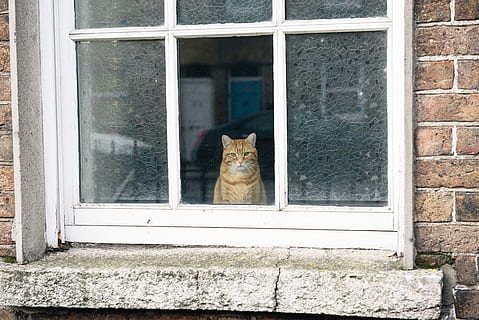
\includegraphics[width=0.9\linewidth]{img/cat_on_window} 
\caption{Query}
\label{fig:searched_scene}
\end{subfigure}
\begin{subfigure}[t]{0.45\textwidth}
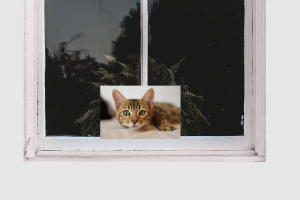
\includegraphics[width=0.9\linewidth]{img/cat_on_window_collage}
\caption{One of the possible collage description for the query}
\label{fig:collage_example}
\end{subfigure}

\caption{Example of searched scene (query) with possible visual description by a collage.}
\label{fig:query_collage_comparison}
\end{figure}

While we were describing the scene, we used words for it. But this chapter with presented solutions do not focus on the search based on the verbal description of the objects. Although, it is one of the possible alternatives to handling problem. Supporting verbal descriptions often require extensively annotated data to use to train neural networks and even though the advancements in the research area it still has a limited ability for extensively described characteristings. Our approach aims to avoid this limitations of vocabulary size semanticization fo the text.. We believe that visually we can capture more diversity. Words often either omit more specific information about the look or are hard to obtain by annotation systems, since the annotation tool may have never seen such combination before. For example, a single word for a human may represent a visually wide range of possibilities, based on clothes, age, and other attributes. We aim to avoid this bottleneck, and we proceed with the search based visual similarities.


In this chapter we utilise approaches for solving known-item search task based on \emph{collage}. Collage $C$ is a (unordered) set of $k$ pictures $C = \{\text{collage\_image}_i\} \text{for}\, i \in \{1, 2, \dots, k\} $.  Each $collage\_image_i$ contains two characteristics: image (i.e., visual description) and spatial information (location). To avoid any scaling and resolution issues, we represent location by a relative offset from the left, top, bottom and right. Therefore, all attributes of spatial information are in range $[0,1]$

This chapter will present three solutions encorporating the pretrained neural networks. To learn more about the networks head back to the chapter \todo{ref}. We start of by a short description of user-program interaction, to more understand the origin of the queries we evaluate on. The chapter invenes the ideas with their evaluation. We test different set of hyperpatameters and investigating their effect on the performance of the system. To check the dataset we work with read chapter \todo{ref}. To know more about the user interface check the documentation in the chapter \todo{ref}. 


\section{User-program interaction}

The query is a \emph{collage} of one or multiple images. Each image also includes its relative position in the canvas.

We provide a user with a canvas where she can place, move and resize the images in the \emph{collage}. Interactively, the set of results is showed (the most similar results). The user can then alternate the query for a new search, or to investigate the displayed results. The figure \ref{fig:query_collage_comparison} shows an example of the query -- the collage of two images (window and cat). 

\section{Solutions overview}

In the rest of the chapter we present different approaches to this task and we test different settings to obtain the best set of hyperparameters. In the figure \ref{fig:processing_pipeline} we can se an overview of the system. The top path is path of the database. The features are precomputed (offline) for all images in the database. We call a \emph{record} an image with it precomputed features. Each of the features may be linked also with additional information. There is one record per input image, but each record may contain multiple feature vectors describing it.

Similarly, for a given collage we extract features by using the same model as for the database extraction. We do that for each of the images in the collage. Since we only need to annotate a couple of images, this can be done online on CPU for most of the networks. In this phase, we have annotated dataset and extracted features from query images. Next, if the records contains multiple feature vectors, we may filter those to decrease the number of vectors we will compare to. We call this process \emph{Relevant Features Extraction}. As a next step, based on the features from the database and the features from the collage compute their distances, i.e., for each query image we compute the distance to each record in the database. The last step, is to merge the rankings, since each of the input images provide us with distances to records in the database. We call this step \emph{Ranking}. In the example image we can see ranking as an average of the rankings for a given record.

We tune several factors in described pipeline. Therefore, we split each step separately and we evaluate it individually. For the next sections we progressively build the pipeline, while describing the particular solutions we used. We start with feature extraction strategies and then we continue with the next steps, which are independent from features extraction.

\section{Features extraction strategies}

In the following section we present three feature extraction techniques. The feature extraction technique defines how we extract features for our dataset as well as for our queries. These obtained features will be later compared agains each other in ranking mechanism. We kick off with the baseline, where we do not use the location of the objects in the collage, only their visual representation. Then we move on onto a solution, which splits the image into regions and compare only to the regions, which relate to the object query. Our last method is experimental and it involves storing a higherdimensional feature vector. This approach aims to test a possibility for no strict cutting, rather computing based on the object location itself.

\begin{figure}[p!]
    \centering
    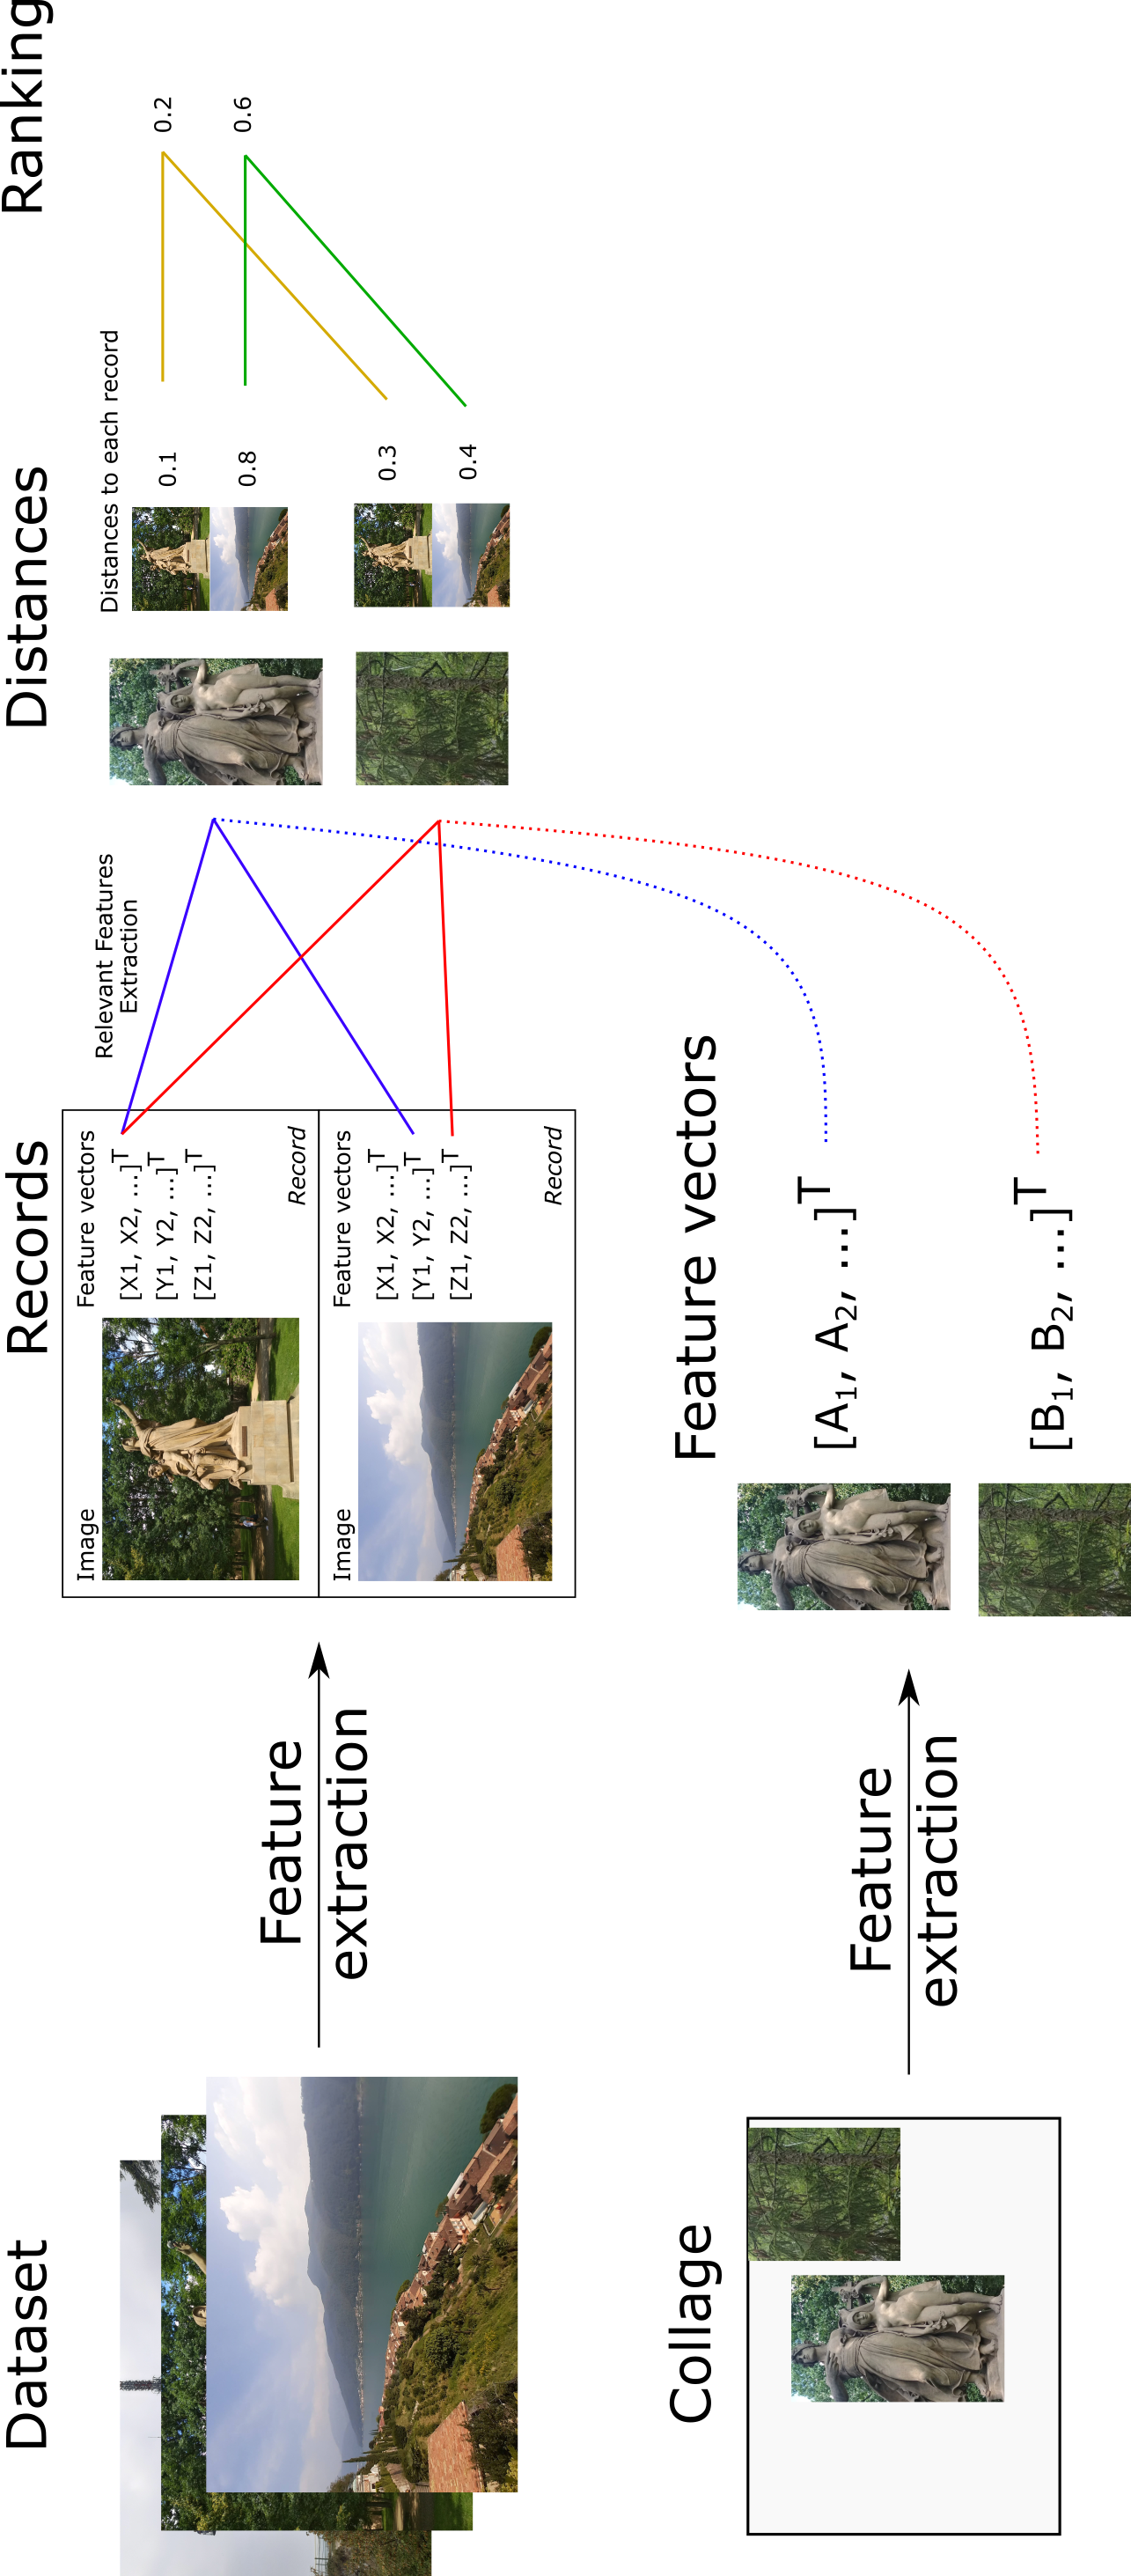
\includegraphics[scale=0.9]{img/features_pipeline_rotated.png}
    \caption{Overview of processing pipeline}
    \label{fig:processing_pipeline}
\end{figure}


\subsection{Baseline -- Image representation}

Firstly, we developed a simple approach, which ignores the information about the position of the images in the collage. We set this approach as our baseline, to see how much we improved a simple solution like this by adding more complexity. For each image in the dataset we compute one feature vector by feeding it to the pretrained convolutional neural network. The images in the dataset are rescaled (without preserving ratio) to fit the input dimensions of the network (224x224).

In the figure \ref{fig:mobilenet_whole_image} we display the performance of such approach on the annotated set of collages. We present the results on the MobileNetV2. We use MobileNetV2 due to its low computability needs and therefore offering quick annotations. It is widely used in the task, where online or near online request time is expected. We included a short description of the network in the Related Works (section \ref{}\todo{ref}).
\todo[inline]{Would be nice to add Resnet50}

\begin{figure}
\centering
\begin{boxedverbatim}
Database:
    - image: 1 feature vector (1 Dimensional)
Query:
    - query_image: 1 feature vector
    - compared to: each feature vector in the dataset
\end{boxedverbatim}
\caption{Overview of the Image representation approach}
\end{figure}

\begin{figure}
    \centering
    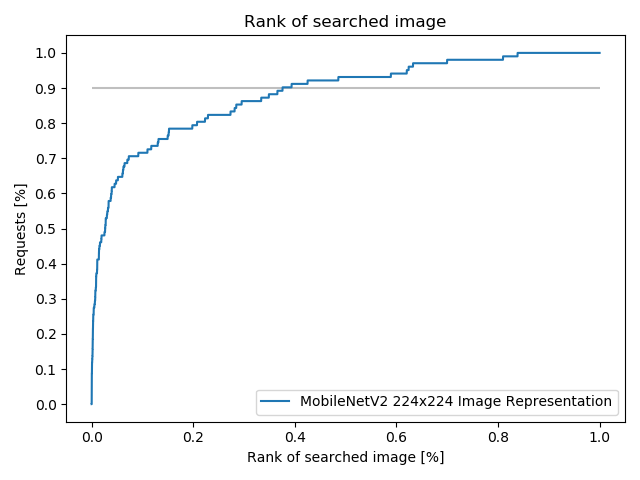
\includegraphics[width=0.8\linewidth]{img/mobilenet_whole_image.png}
    \caption{Performance of MobileNetV2 on annotated collages}
    \label{fig:mobilenet_whole_image}
\end{figure}

\subsection{Splitting an Image into Regions}

Our goal in the next presented solutions is to use also the information about objects' location. Our dataset contain many different images, with objects in different positions. Although, as we have seen in the previous section, comparison to the whole image worked well. Here we propose to include higher granularity and to split the image into multiple regions. That way we can compare the query images only to the region which is interesting (for example, if the tree is placed in bottom right corner, we would compare only to the region from bottom right corner). If we cut each image to the same regions, we will be also able to speed up the processing.

We define a cutting into a regions. Each record contain one image, which is visually divided into  $N \times M$ regions. Then for each region we compute a feature vector via pretrained model. When the query comes, we will compare the query feature vector only to the regions from the record, which overlap.

\begin{figure}
\centering
\begin{boxedverbatim}
Database:
    - image:
        - Multiple regions:
            - region coordinates
            - feature vector (1 Dimensional)
Query:


    - query_images: features vectors from M
    - compared to: only to related crops from each image
\end{boxedverbatim}
\caption{Overview of the Regions' approach}
\end{figure}



\subsubsection{Regions Shape}

In order to use transfer learning for common CNN and to avoid additional skewing in resizing, we limit to the regions only to the shape of squares. Since this input size of the square is one of the parameters, we aim to use the size of the squares the same as the size of the input of the network. This helps us to avoid unnecessary scaling which may be introduced when the length of the side of the square does not match with the input for the network.

A second limitation we create is for the regions to fully cover the record image. Since we now know we need square regions which cover a full image, there might be no way to cut image into the regions without any overlapping. Therefore, we create enough regions to fully cover the image and we split the excess between the regions. This excess is evenly distributed over the regions, creating equal overlaps. We split based on the predefined number of regions, since the number of regions results in the multiplicative coefficient for the complexity.

Allowing overlaps plays another role in this solution. With the rigid frame without overlapping, it could happen, that they would split an object into two parts. With overlaps, we know that some part is shared between both regions.

Our fixed parameters are input shape width $s$ and the number of regions we want to use $N \times M$ and image size $h, w$. We solve the task of choosing regions splits for one axis, the second is done equivalently. We know, that the last region has to end with the edge of the image. Therefore the starting coordinate of the last region is $h - s$. We then split the remaining "space" over axis over $N-1$ regions equally. We call this distance $step$, since it says the distance between the regions. The starting coordinate $r_i$ of the $i$-th region in a given axis is:

\begin{align*}
step = (h - s) / (n - 1) \\
r_i = {i \, step\,\text{for}\,i \in \{1, 2, \dots, N\}}
\end{align*}

With the condition on full coverage of the image (i.e. \(s N >= \text{h}\), and for $M$ respectively) we obtain full coverage of the image by the regions. Overlaps are evenly distributed over both axis. Although, with a bigger sized regions overlaps may occur between more than 2 regions. For example, if we split an image with width 180 into three regions with width 96 pixels, some areas of the image will be included in all three regions. This happens, when the $step <= 2 s$.

We evaluate the performance of the same network using a different number of regions. This experiment is shown in the figure \ref{fig:different_number_regions}. In the same figure we also show the effect of increasing the region width.

\todo[inline]{missing based on different size, since it was not preprocessed}
\begin{figure}
\centering
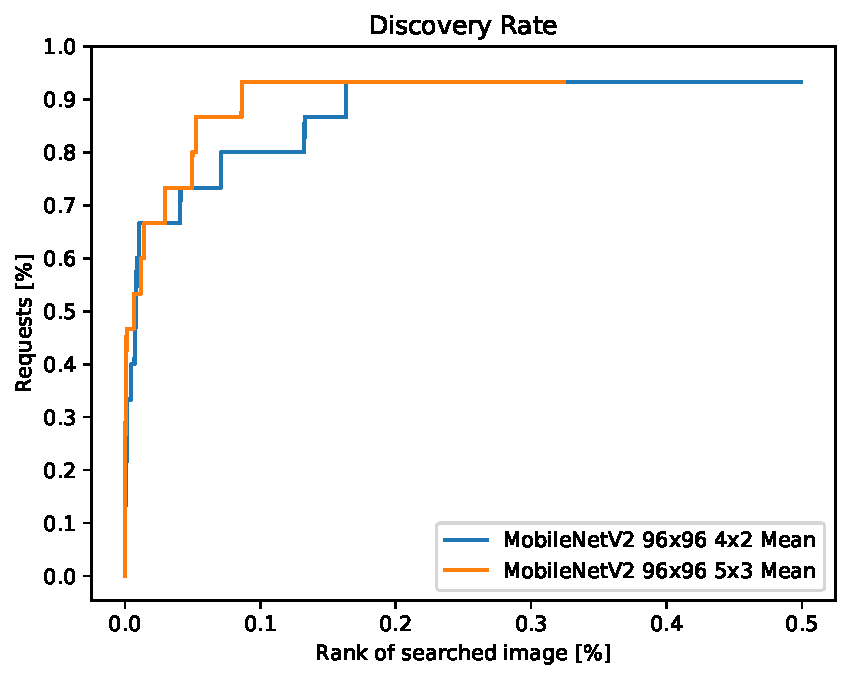
\includegraphics[width=\textwidth]{graphs/78f2a977489ac08dddac6f53446b388292306ec95f9dcbc7ca8359fbedfed9b0}
\caption{An experiment comparing the offect of the regions size and the number of regions.}
\label{fig:different_number_regions}
\end{figure}


\subsubsection{Choice of regions}

Given one incoming query image with its position and shape we propose several methods for choice of the “targeted” regions. For each one of the fixed regions we compute %\[\text{IoU_{i,j,k}} = \text{IoU}(Ri,j; Qk) for all i, j. \]

First of the options, is to only compare the region with highest Intersection over Union, limiting to the argmax IoUijk. I.e. for each i belongs I only one region would taken into account.

Second approach is to collect all intercepted regions for the similarity. This is an exhaustive process. This may result in increased computation time, i.e. usually from 2 to 9 times slower. In case of a huge set of data without any indexing, it may increase time of a request from 1 sec up to several seconds.

Third choice is to limit the number of targeted regions to a certain number. This offers us an advantage of fuller coverage and possibility for better match in neighbouring region, on the other hand provides an upper bound for the computational time required per request. 

Visualisation of chosing different number of crops can be seen in figure \ref{fig:fish_with_grid}. A comparison of the performance dependend on different number of chosen crops is shown in figure \ref{fig:crop_limitation}.

\begin{figure}
\centering
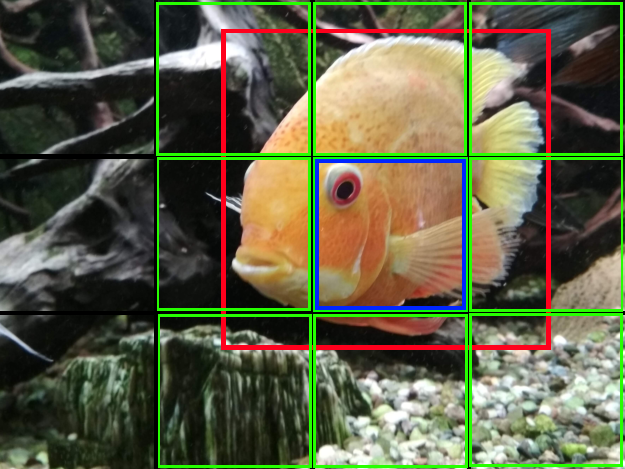
\includegraphics[width=0.6\textwidth]{img/fish_grid_regions}
\caption{Example of choosing the corresponding regions. Red: query position; Green: all intercepted regions; Blue: region with highest IoU.}
\label{fig:fish_with_grid}
\end{figure}


\begin{figure}
\centering
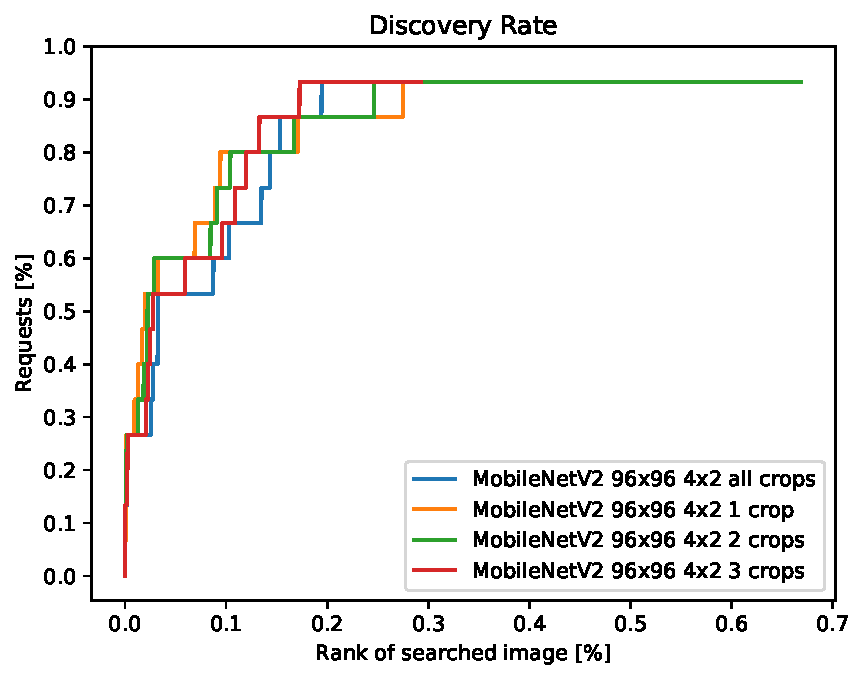
\includegraphics[width=\textwidth]{graphs/c2cf4e147040018e6cfc46043bb59de4f5f3e83441c1e1024af0b7bab644a994}
\caption{Performance of the system based on different number of chosen crops}
\label{fig:crop_limitation}
\end{figure}


\subsection{Using more information from antepenultimate layers from CNN}

The previously mentioned approach has a shortcoming. It is not able to grasp the arbitrary position of the object, rather it has limitations to previously fixed regions. This may lead to decreased performance for the objects, which cover a bigger part of the scene, i.e. in the previous case, it may overlap over multiple regions. This brings not only computational disadvantages but also reduces the amount of information which are used when compared to the query.

We propose an approach, where an antepenultimate layer of common CNN's may be used. Common CNNs are built out of several building blocks, i.e. convolution layers intervened by pooling (TODO image). This approach proved its ability for image recognition and many other related tasks (TODO add source). Many of the current state-of-the-art models use the pooling layer before fully connected layer for categorization.

We aim to leverage this antepenultimate layer, which contains not only visual features but also spatial information.

\begin{figure}
\centering
\begin{boxedverbatim}
Database:
    - image:
        - feature vector (3 Dimensional):
    - model M
Query:
    - query_images: features vectors from M, then average pool)
    - compared to: average pool over selected region for item 
                   in the database
\end{boxedverbatim}
\caption{Overview of the Spatial approach}
\end{figure}


\subsubsection{Choosing region of interest in the layer}

Layers before pooling on which we focus are 3 dimensional. First two dimensions contain spatial information, which is propagated from the previous layers. The third dimension contains visual information.

In order to obtain only a part of this layer we are interested in (i.e. our query was placed in that specific region) we need to take only a subset over first two dimensions. For a query defined by Qi = (y, x, h, w) and layer Li with first two dimensions H, W we consider a Li[y * H, x*W, (y+h) * H, (x + w) * W]. 

It is important to notice, that these layers use to have significantly lower height and width, compared to the input of the network. For example, before-last-pooling layer of Resnet50V2 has dimensions (7,7,2048). Therefore, we round our subset to nearest whole number and in case of no intersection we maintain at least intersection of size 1x1.

After this choice of the region of interest, we continue with the pooling layer in order to obtain one feature vector.

In comparison with the previous Splitting in regions approach, we see an enhanced ability to grasp more variability in object position. Especially, in queries which overlap most of the regions. On the contrary, this approach may require more memory, as for comparison for Resnet50V2 with 12 regions we needed to work only with 12 feature vectors. With the before-last-pooling layer we need for Resnet50V2 to work with 49 feature vectors. This may not be limitation with smaller feature vectors, but may come as a practical limitation based on the size of the dataset and computability power available.


\section{Ranking}
In the previous sections, we talked about the obtaining feature vector for the items in the database of the regions we are interested in. In this section, we take a closer look on further processing these obtained feature vectors.

Assuming we have an image for the query, we use the same model to compute the feature vector as was used to precompute the features for the database. Based on that we define a distance D, as the distance between the feature vector of the query and feature vector of the item in the database. This comparison to each database item gives us the distance between each item in the database and our query image.

Based on these distances we order the results, starting from the lowest to the highest distance. This distance acts as an inverse for the similarity. Similar to the results are, lower is the distance.

We use 3 main distance metrics:
Cosine Distance
Euclidean L2 distance
Euclidean L1 distance

\section{Multiple objects in the scene}

So far we talked only about handling queries consisting of one searched object. This limitation is very strict and therefore we experiment with multiple approaches to index the database based on multiple objects in the scene.

Firstly we make an assumption, that all query images have the same importance and are expected to be with the same level of relevance. Therefore we approach this problem as a set of query images, rather than as an ordered list.

We work further only with already precomputed rankings with corresponding distances for each image/part of the image. We propose several ways to merge the rankings.

We define ranking $R$ as a set of distances between the query image $q$ and database item $i$. We look for a function $r: R^n \rightarrow R$, which merges multiple rankings into one final ranking. Our goal is to minimize rank for each of the queries in the test items.

We tested several functions for this role and to compare a function that does not take into account the distances with different functions over the distances. A comparison for MobileNetV2 can be seen in figure \ref{fig:ranking_funcs}.

\begin{figure}
\centering
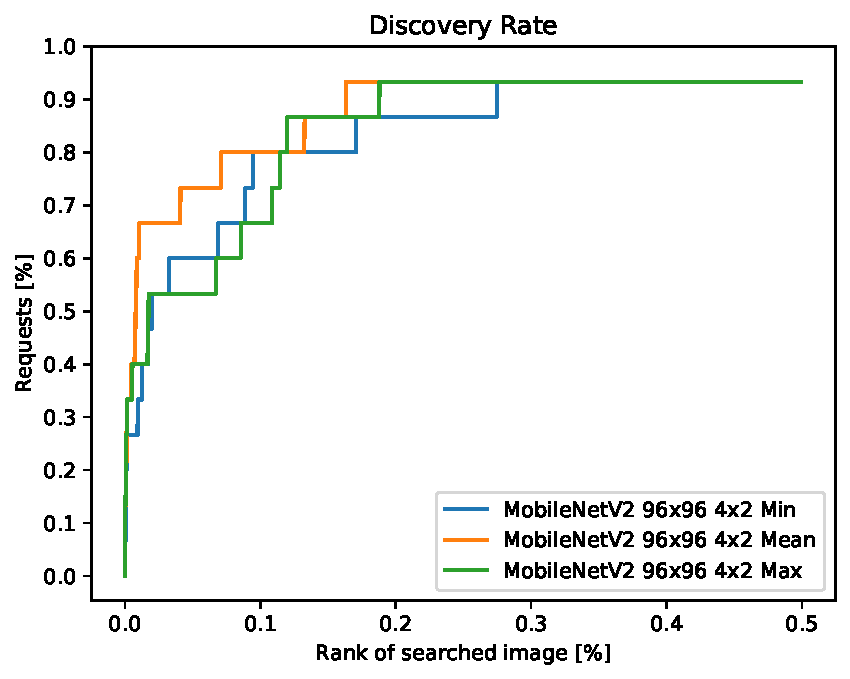
\includegraphics[width=\textwidth]{graphs/362cb9a687ce05c7732f973defca88fb8c5c393f5992066521343314698c9de7}
\caption{Performance of the system based on different fusion method}
\label{fig:ranking_funcs}
\end{figure}

\section{Padding}

Our input images provided by a user do not have to be a square images. Although, we need to prepropress these to obey the input shape of the feature extraction model we use. These models use usually square shaped input. In our case, we compare the performance of the solution based on three different approaches on input reshaping. We compare padding the input with black or white and our third option is rescaling the images. Rescaling is done in the manner, where distortion occurs for non square images, i.e, a tree becomes shorter and wider, and the car becomes narrower and taller. The results are available in the figure \ref{fig:TODO}

\section{Dimensionality reduction}

In the previous sections we evaluated several hyperparameters of the system to achieve the best performance. In this section we take a look in reducing the dimensionality of the extracted features. The extracted features from the neural networks with removed last fully connected layer are often high dimenisonality data (for MobileNetV2 its 1024 features, for Resnet50 it is 2048 features). Even though we were able to test the hyperparameters without introducing another factor -- dimensionality reduction -- we want to test also if such reduction can have also positive effects.

\todo[inline]{Mozno viac popisat PCA?}

We perform Principal Component Analysis on the extracted features. We evaluate the effects of the PCA given different number of extracted components. This helps us to significantly reduce the size of the dataset used and therefore offers us a solution with good scalability.


\chapter{Search by Face Similarity}
\label{ch:face_search}

In this chapter, we propose another approach to the \acrshort{kis} task. This approach focuses only on the case, where the images include people.
We investigate the option of finding the target image based on the person's face in the image and other faces in the dataset.

This approach arises from practical reasons. Once we investigated the V3C1 dataset, we realized that in many of the images are people. We can use the previously investigated approaches based on the location and visual similarity to find the target image. However, with the increasing number of images showing people, it becomes difficult to retrieve the correct target image. Simply searching for a person in the top left corner would retrieve all images with a person in the said corner (not just the one we are looking for). Also, finding a good representative face with similar background becomes a challenging task.

In this chapter, we aim to provide a search mechanism employing finer features of one's face. We provide a simple search structure to investigate the faces in the dataset.

We first extract the faces from the dataset, and then we obtain a descriptor for each one of them. Based on these descriptors, we organize the faces into a traversal structure supporting navigational commands.

The task of comparing faces of the people and saying which look more similar has its roots in the human perception of faces. Therefore, to evaluate the individual steps, we conduct experiments with human subjects.

Our experiments suggest that the feature space of the descriptors has a limited power to sort people based on the similarity in a way people do. Based on that, we implement the traversal structure, which can be used with the presented descriptors or any other descriptors of the faces that could be developed in the future.


\section{Overview}

Our goal is to propose a traversal structure based on the faces found in the dataset. Ideally, we would like to group similar faces so that users can quickly decide if the group of people corresponds to the target face they look for, or not.

% We, as people, do not perceive the similarity of faces always the same way. We hypothesize that when we two people find the most similar faces to a given face, they will not choose the same set. We verify this hypothesis in the case study, presented in section \ref{s:case_study}.

The question we ask in the following sections is if the face descriptors can sort people based on the similarity, similarly to human perception. If yes, then we can argue that traversal structure based on these face descriptors may help. We leave experiments with additional descriptors for future work. In our case, we compare only one type of face descriptors to human perception, although, in future work, it may be experimented further with other descriptors.

% If we do not observe any correlation between the ordering based on the descriptors and survey responses, then the descriptors would not be able to group similar faces as people do.

\section{Extraction of the faces}

If we look at the dataset, we notice that only a small portion of the people look directly into the camera. Since the images come from the videos, most of the people captured are doing some activity and not looking directly into the camera. As discussed in section \ref{s:dlib}, we select the \acrshort{cnn} based approach to extract the faces since it worked better with a wider variety of poses.

For our experiment, we use only a part of the original dataset. We extract faces only from the first 316 videos of the V3C1 dataset. Again, we firstly use image extraction from videos (refer to section \ref{s:dataset}), and only then we extract faces from images. 

From these 316 videos, we were able to extract more than seventeen thousand faces. However, after investigation of the dataset, we found out that many of the extracted faces had too low resolution. The majority of the extracted faces did not even cover 5\% of the image. Therefore, we decided to filter out the dataset further and remove all the faces that did not cover at least ten percent of the image. The distribution of the area covered by a face is displayed in figure \ref{fig:faces_size_distribution}. After the filtering,  we obtained 2047 faces from the 316 videos. A random selection of faces is shown in figure \ref{fig:random_selection_faces}. 

We then visually investigated the extracted faces. The dataset contains people of different ethnicity, age, and gender. The faces are displayed from a wide range of angles, including even full side views. Some of the people wear glasses, headphones or other accessories. The dataset also contains some pictures of children. The model also extracted a few drawn faces or faces of sculptures.

% Because most of the faces cover at least 5\% of the image, we decided to filter out too small faces. We filtered out the faces, which covered less than ten percent of the image.

\begin{figure}
    \centering
    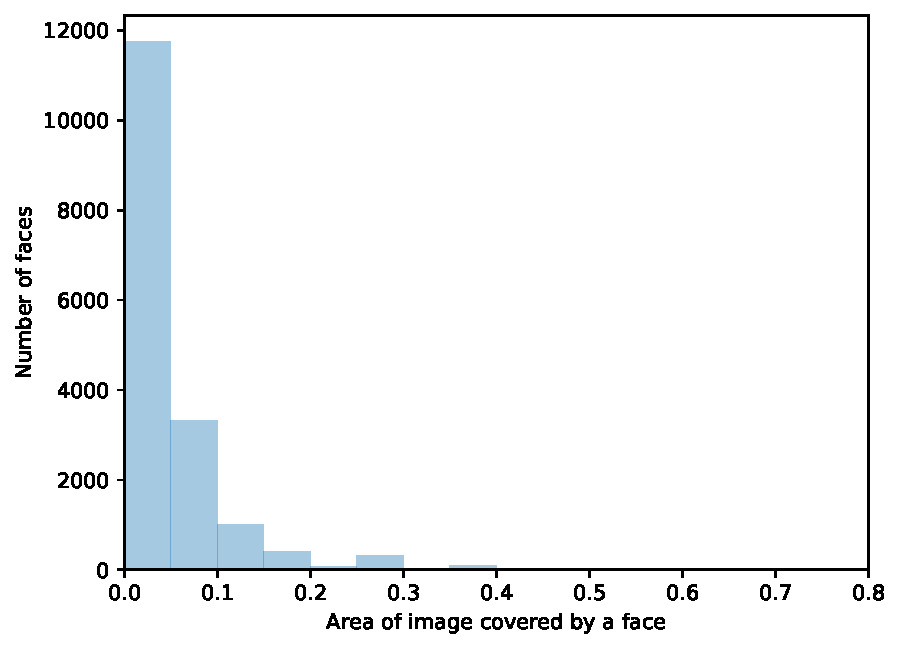
\includegraphics[width=0.7\linewidth]{graphs/faces_size_distribution.pdf}
    \caption{Area of image covered by a face}
    \label{fig:faces_size_distribution}
\end{figure}

\begin{figure}
    \centering
    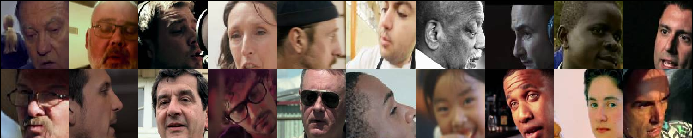
\includegraphics[width=0.98\linewidth]{img/random_selection_faces.pdf}
    \caption{A random selection of faces extracted from the dataset.}
    \label{fig:random_selection_faces}
\end{figure}

\section{Face similarity based on the deep features}

For extracting descriptors (i.e., feature vectors), we use the dlib pre-trained model, as discussed in \ref{s:dlib}. The network outputs vectors from space $\mathbb{R}^{128}$. We use the output of the network directly as our feature vectors. 

Note that often \emph{face features} refer to the specifics of the face landmarks, the color of the eyes, size of the lips, etc. To avoid confusion, we use the term \emph{face encoding} or descriptors for feature vectors obtained by the neural network. Such face encodings are usually from the space $\mathbb{R}^n$, in our case $n=128$.

After obtaining the face encodings for our dataset of 2047 faces, we were interested in if this feature space, created by the \acrshort{cnn} is able to sort the faces based on the similarity in a way people do. 

The library, from which we use the model, refers to a threshold 0.6 in the euclidean distance as the threshold with the highest accuracy on the verification task. The example of the closest faces based on this threshold is displayed in figure \ref{fig:closest_faces}. The top left image belongs to the target face. In the provided example, we can see that the face encodings close to our target face truly belong to the same person. Unfortunately, we can see, that with increasing distance other people appear even below the threshold 0.6.


\begin{figure}
    \centering
    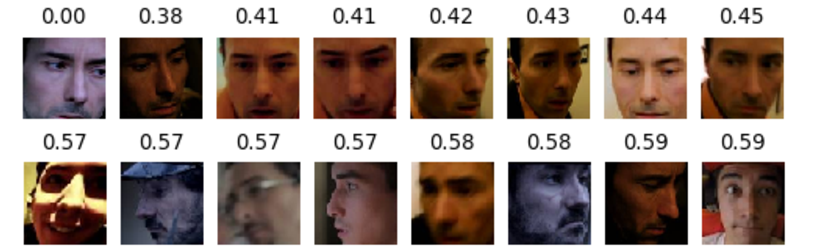
\includegraphics[width=\linewidth]{img/man_closest_faces.pdf}
    \caption[Examples of the retrieved closest faces to the target face based on euclidean distance]{Examples of the retrieved closest faces to the target face (top left) based on euclidean distance. The number above each image represents the distance from the target.}
    \label{fig:closest_faces}
\end{figure}

\section{Case study}
\label{s:case_study}

% We want to find out if the space of the obtained face features, can order faces based on their similarity similarly to human subjects.

In this section, we investigate a possible correlation between the given faces as perceived by humans and the distances between their encodings.

We conducted a study with 25 participants. We presented to them a $10\times10$ grid of randomly selected faces from the dataset. 
Then we showed them ten randomly selected target faces of different people (same set of faces to each participant). We asked the participant to select for each target face \emph{exactly} three faces from the grid that looked the most similar. 

%Then we asked them to select exactly three faces, which are the most similar to the provided target face. Our test contained ten randomly pre-selected faces of different people. Out of 10, one of them was a child, we estimate below ten years old. Two of the other target faces were present in the grid.

Out of 10 target faces, three were also represented in the grid. Two of the faces were extracted from the same image, i.e., the same angle of the face. The third face, which was also present in the grid, had two representants in the grid. First identical to the target face and the second with only a minor change of the angle.

Firstly, we investigate how likely it is that the human subject notices that the face they are looking for is also present in the grid. In the first case, twenty-four out of 25 respondents selected the face corresponding to the same target person. In the second case, only 20 respondents found the face in the grid. We assume that the first case was ``easier'' because the face comes from black and white image, therefore, was easier to notice. In the third case, two face views of the target person were available in the grid. Nine respondents selected both correctly, and eleven respondents selected only one of them. 

As our next step, we empirically evaluate, if the model used for obtaining the face encodings, can sort the faces based on the distances similarly as human subjects do.

We further investigate the seven target faces, which were not present in the grid. Excluding the three cases, where the target face is in the grid, we avoid overestimating the quality of our model, since we know, that the model is performing well on the verification task. For every face $F$ from the grid $G$, we compute the euclidean distance from the target face $T\in D$, where $D$ denotes our dataset of faces (between their encodings). We then reorder the faces from the grid based on this distance (similar to the ranking from the previous chapters). 

Formally we define distance $\gamma$ between faces $F, F' \in D$ based on the descriptor extraction function $f$ and euclidean distance $d_e$:

$$
\gamma(F, F') = d_e(f(F), f(F'))
$$

This definition allows us to rank faces in the grid $G$ based on the target face $T$:

$$
    r_T(F) = |\{F'\in G\mid\gamma(F', T) < \gamma(F, T)\}|
$$

Again, to ``break ties'', we use any arbitrary total ordering $<_F$ over faces, as in \autoref{s:task_formulation}.

% \todo{chyba kucerava zatvorka}
% $$
%  r_T(F) = |\{F'\in G\}| \gamma(F', T) < \gamma(F, T) \lor (\gamma(F', T) = \gamma(F, T) \land F' <_F F)\} |
% $$

% The closest face has the lowest index. We refer to the face's index in the sorted set of faces as $rank_t$ with respect to the target face $t$.

Note that this ranking function is a bijection between the faces in the grid and a set $\{0, 1, \ldots |G| - 1\}$, given the target image. Therefore, it is reversible, i.e., we can obtain the face from the given rank. Based on this ranking, and the data obtained from the respondents, we aim to verify the correspondence of the ranking based on distances of the encodings and the most similar faces as identified by the respondents.

This allows estimation (based on the results of the survey)  of the probability $p$ that for given target face $T$ user selects a face with rank $R$. We also denote the number of respondents that selected face $F$ for target face $T$ as $N_T(F)$. The resulting probability then is:

$$
    p_T(R) = \frac{N_T(r_T^{-1}(R))}{25}
$$

Finally, to provide comprehensive overview, we compute combined probability of selecting face with rank $R$ by combining the results for all target faces $\mathcal{T}$:

$$
p(R) = \frac{1}{\abs{\mathcal{T}}}\sum_{T\in \mathcal{T}} p_T(R)
$$

Note that as each user selects three faces, it holds: $\sum_{R\in\{0,1,\ldots99\}} p(R) = 3$.

We plot the empirical probability $p$, of a user selecting the face on the $k$-th rank, given the target face. If the user is fully coherent with the model, they would choose the closest three faces based on the euclidean distance, and for the $R \in \{0,1,2\}$ we would see a probability $p(R) = 1$ and zero otherwise. 

This plot of the probabilities is displayed in figure \ref{fig:survey_distribution}. We do not normalize this plot, so we can talk about the probability, given our experimental settings, i.e., selecting exactly three faces.

% In the same figure \ref{fig:survey_distribution} we can see the distribution only of the seven presented faces.

% In this experiment we excluded a target face, which belonged to a child (the only child among the 10 target faces). \todo{}.

We are interested in the distribution of ranks given the faces selected by the users. We want to know if there is any correlation between similarity in the feature space and the similarity perceived by the human respondents. 

% From the survey responses we create a heatmap for each task. The size of the heatmap corresponds to the size of the face grid, i.e., $10\times10$. The element on the position $task, i, j$ of the heatmap corresponds to the number of times, the face at $i$-th row and in $j$-th column was selected in the given $task$. We use the heatmap and the ranking based on the distances in the feature space, to compute, how many closest faces from feature space were actually selected. We do the same for each rank. The normalized results over all possible ranks (from 0 to 99) are plotted in the figure \ref{fig:survey_distribution}. If the users perception was fully coherent with the ordering based on the distances in the feature space, the  
% probability on the first three ranks (0,1,2) would be equal to 1. Even though we do not see such full coherence in the results, we can see a trend of decreasing probability of choosing a face by user with the increasing distance from the target face.

% We also show a comparison to the performing only six tasks, excluding the one, where the target person was child. The used network for feature extraction as many other are not performing well on the children from the dataset. This is caused by fact that most of the available face datasets contain only adults. This causes the networks to often put children closer together, even though, they may be a different person. Encodings of two different children tend to be closer to each other compared to the encoding of the two adults (source: \href{https://face-recognition.readthedocs.io/en/latest/readme.html#caveats}{Face Recognition Caveats}). Therefore we can see a significant improvement over the lowest ranks, since selecting a child from the map resulted in smaller distances, compared to the adults.

As the last investigation from the case study we provide a graph (figure \ref{fig:cumsum_faces}) displaying the expected value of the number of faces $X_R$ selected up to rank $R$, which can be expressed in terms of $p$ as $\mathbb{E}[X_R] = \sum_{R' \leq R}p(R')$. On average, one of the three selected faces by the user has a rank of less than 12. In the plot, we also present a ``random selection''. This would be the case of no underlying information on the face similarity from the model. Therefore, users would be equally likely to choose face at any given rank.

We leave for future work, a more comprehensive study with more target faces providing more reliable estimates. Based on the experimental results of this user study, it seems to indicate that the distance over encodings correlates with the similarity of the original faces as perceived by the human subjects.

\begin{figure}
    \centering
    % \begin{subfigure}[b]{0.48\textwidth}
    %  \centering
    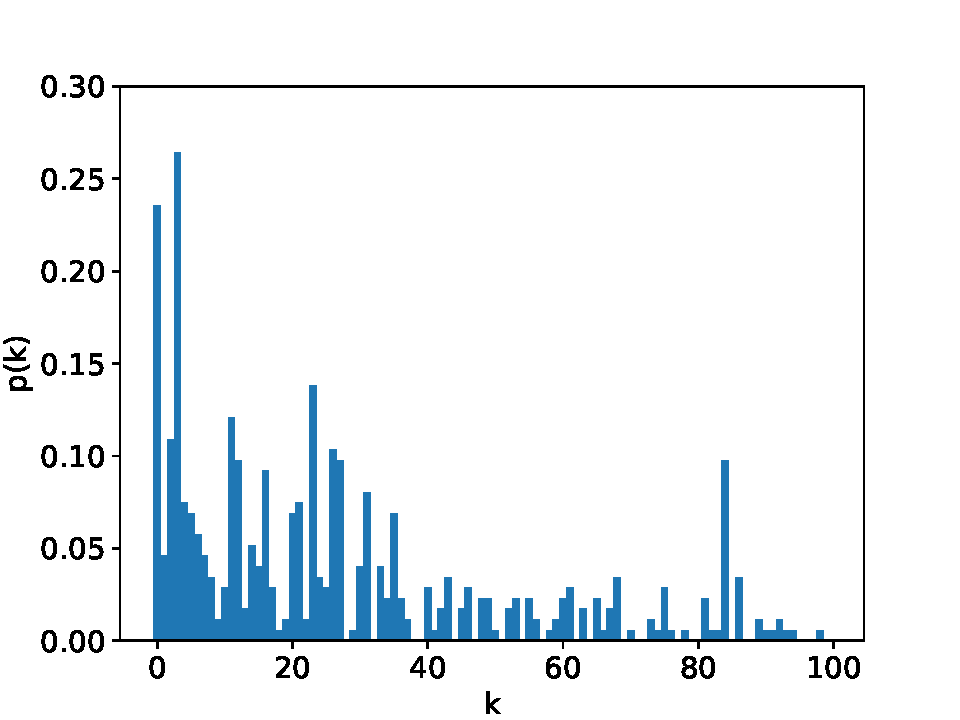
\includegraphics[width=0.6\textwidth]{graphs/survey_distribution_without_the_easy.pdf}
    % \caption{Performed on seven tasks, which did not contain the target person in the grid}
    % \label{fig:survey_all}
    % \end{subfigure}
    % \begin{subfigure}[b]{0.48\textwidth}
    %  \centering
    %  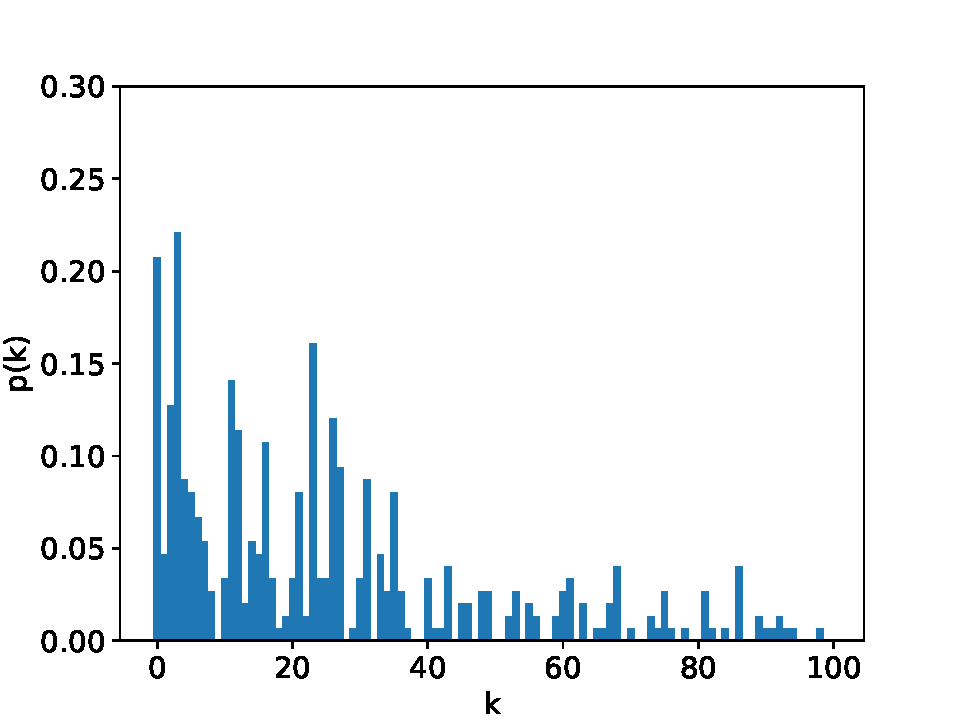
\includegraphics[width=\textwidth]{graphs/survey_distribution_childless.pdf}
    %  \caption{Performed on six tasks, extracting the task involving a child}
    %  \label{fig:suvery_childless}
    % \end{subfigure}
    
    \caption{Collected statistic on how likely user selects $k$-th closest face to the target in the face grid}
    \label{fig:survey_distribution}
\end{figure}


\begin{figure}
    \centering
    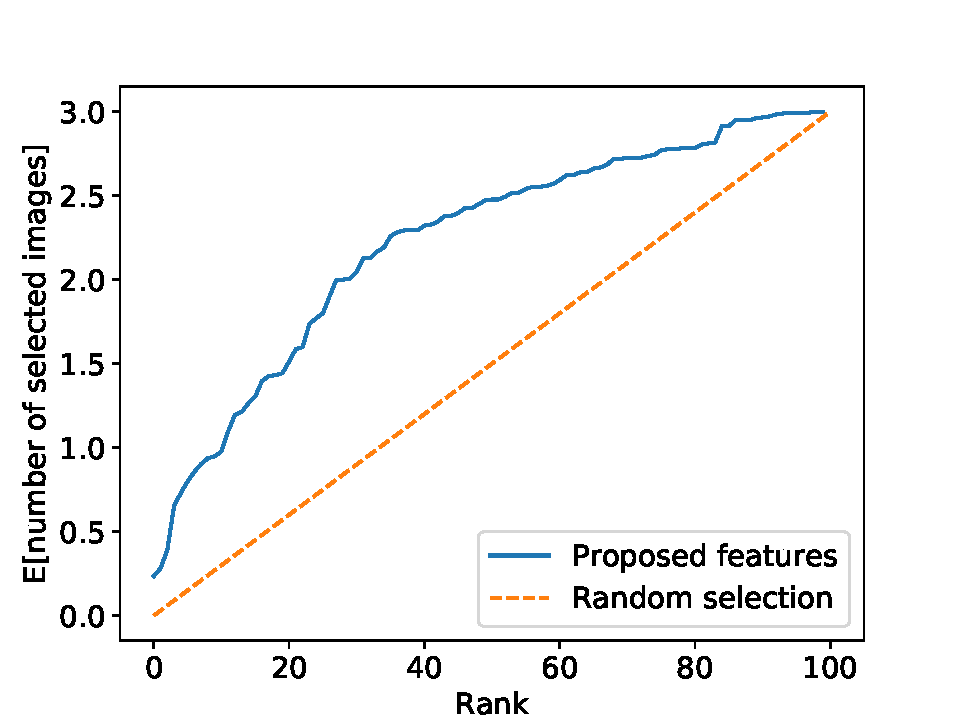
\includegraphics[width=0.8\linewidth]{graphs/survey_cumsum_without_the_easy.pdf}
    \caption{Expected value of the number of images selected up to a given rank.}
    \label{fig:cumsum_faces}
\end{figure}

\section{Building a traversal scheme}

In the previous sections, we extracted and encoded faces. In the case study, we investigated the feature space for the correspondence to the human annotations. Here we propose a solution of organizing faces into a multilevel view. 

As we discussed in \autoref{ch:related_work}, a common solution for the traversal system is a 2D grid.  In the 2D grid, a user can navigate using the following commands: move left, right, up, and down.


% This usually allows users navigation queries, as left, right, top, bottom. We call a set of images, which is visible at a particular step a \emph{display}. The display may contain tens to hundreds of images at once, depending on multiple factors, e.g., a user's screen size and the size of the displayed image.

Since most of the time, we want to browse more than a hundred images, it becomes inconvenient to preview dataset only in one layer. Therefore, we build a simple multilevel structure to ease the navigation.

\subsection{Tree-based structure}

Our goal is to organize a dataset of images $D$ to allow easy navigation. Let us assume that the dataset can be organized into a grid of size $N\times M$. We leave the choice of specific dimensions to the user. We prefer a square setting, although it is not required. In case that the size of the dataset $|D|$ is not square of any number, we recommend adding a placeholder images.

We organize (so far in a non-specific way) the items from the dataset into a chosen 2D grid. This is the base layer for the tree structure, we denote this grid as $L_0$. The layer has dimensions $L_{0, h}\times L_{0, w}$. Based on this layer, we create the next layer as only a subset of this layer. Firstly, we select $k$, which represents the sampling size factor. It means that every $k^2$-th image is selected as a representant to the next layer. The overview of the structure is shown in figure \ref{fig:tree_structure}. 

The layer $L_{i+1}$ has $1/k$ of the size in both axis of the $L_i$, more specifically, if the $L_i$ is of the dimensions $L_{i,h} \times L_{i,w}$, the layer $L_{i+1}$ has following dimensions:

$$
    L_{i+1, h} = \ceil*{L_{i, h} / k}
$$

$$
    L_{i+1, w} = \ceil*{L_{i, w} / k}
$$


The item on the position $m, n$ in the $L_{i+1}$ is replicated from the layer $L_i$ as follows:
$$
    L_{i+1, m, n} = L_{i, mk, nk} 
$$

We continue reducing the size of the layers until the layer will fit into a single display.

In this structure, we support six types of navigation: left, right, down, up, in and out. In and out represent operations of traversing between the layers and other directional commands allow navigation  within the layer. 

\begin{figure}
    \centering
    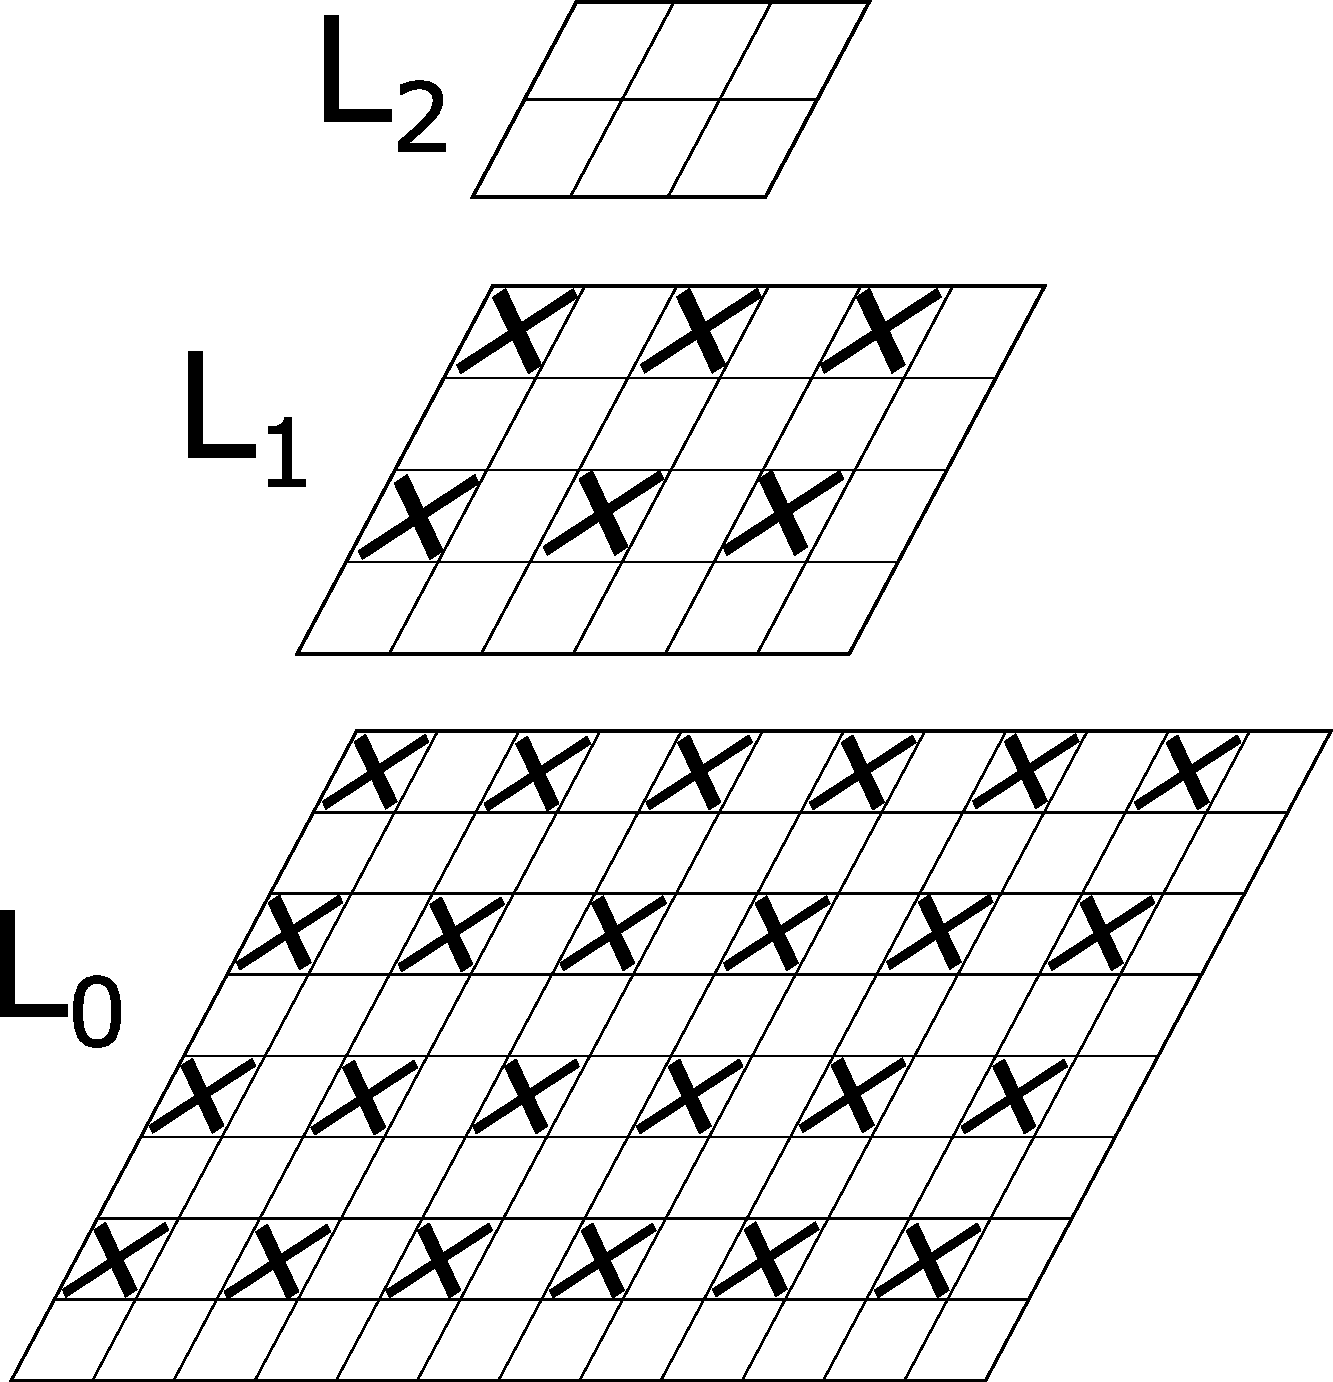
\includegraphics[width=0.3\linewidth]{img/tree-structure.pdf}
    \caption{A preview of the tree-based structure with $k = 2$ for previewing images. The marked items are selected for the layer above as representans.}
    \label{fig:tree_structure}
\end{figure}

\subsection{Bottom Layer -- Self-organizing map}

In the bottom layer, we would like to make use of the face encodings. As we reviewed in \autoref{ch:related_work}, Self-organizing maps showed a promising way to project high-dimensional data onto the 2D grid. We train a self-organizing map on our dataset of face encodings. For our particular dataset, we train a network of size $50\times 50$. This offers us 2500 neurons, having more neurons than there are faces in the dataset.

To train a \acrshort{som}, we use a MiniSom framework \citep{vettigli2013minisom}. We use the default setting for the SOM, a gaussian neighborhood function with an asymptotic decay for the parameters. This setting showed the best results after visual inspection. We train the \acrshort{som} for 200\,000 iterations, i.e., each example was seen on average 100 times during the training. Since the training of the \acrshort{som} highly depends on the random initialization, we first run the same settings for ten different seeds for 30 000 iterations. Based on the results, we selected a seed with the lowest quantization error (refer to \autoref{s:som}). We reran the training with the best seed and trained for 200\,000 iterations.

\begin{figure}
    \centering
    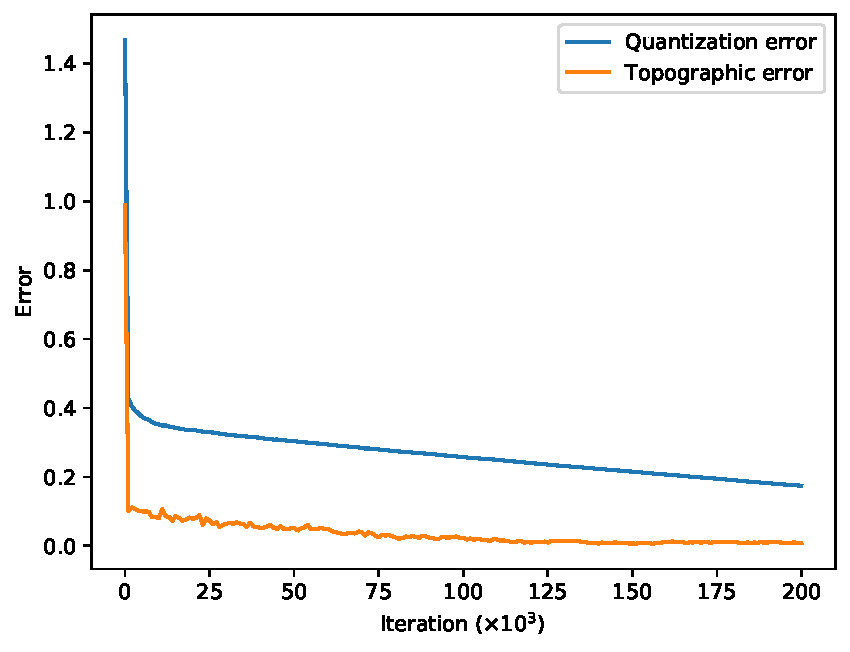
\includegraphics[width=0.8\linewidth]{graphs/som_errors.pdf}
    \caption{Training $50\times50$ SOM, 200 000 iterations.}
    \label{fig:som_training}
\end{figure}

The training errors are shown in figure \ref{fig:som_training}. We can observe that topographic error is at this stage stable. Even though the quantization error has not converged yet, at this stage, we did not achieve any improvements by our visual inspection.

Then we built the bottom layer for our traversal structure based on the trained SOM. This SOM represents our grid. For each neuron in the SOM, we assign a face whose encoding is closest to the given neuron's weight vector. We refer to this face as a representative of the given neuron.
Note that this way of selecting representatives does not avoid duplicates (i.e., assigning the same face to multiple neurons). 

We explored the assignments, and these are the observations we made: 345 faces out of original 2047 is not assigned to any of the neurons. However, only 22 out of these 345 faces have the distance to the closest face which is assigned to a neuron, higher than 0.45. In the original study, the authors of the model suggest considering encodings closer than 0.6 to be of the same person. As our investigation of the dataset in the figure \ref{fig:closest_faces} shows, threshold 0.45 is strict for assigning the same person. Therefore, we expect that those 323 faces missing represent a person, which is already among the representants. The maximum distance for the excluded 22 faces is 0.56, which is still below the initially proposed threshold for assigning the same person. Nevertheless, we verified that all of these faces, which are not selected as representants to any of the neurons of the \acrshort{som}, are still accessible from the structure by an additional utility that shows the most similar faces to a given face. We discuss this utility in the next section.

\subsection{Accessing the most similar faces}

We enhance the tree-structure to support displaying the most similar faces to a given face. A user can click on any of the displayed faces. Images, which contain a face considering to be the same person (threshold 0.6), are then displayed. This is helpful to find the exact target image when the user finds the same person on the map. This also provides a way to learn for the user. The user can display close faces, and investigate the characteristics by which faces are grouped by. Based on this, the user can utilize information about the structure to perform the face search faster in the next searches.

\section{Summary}

Our experiments suggest that the space of encodings contains some information on the face similarity. We propose a multilevel structure to explore a dataset of faces. In this structure, we support navigational commands that allow users to navigate within a layer (move left, right, up, and down) as well as traverse between the layers. Lower layers contain more faces, while upper layers offer a greater variety of the displayed faces.

We created the bottom layer with the help of a self-organizing map. We assigned each neuron its closest representative from the dataset. To provide users with additional insight into the data, we also support a search for closest faces to any given face in the traversal structure.

In the last section, we present a preliminary evaluation. More thorough evaluations, with more participants, would be needed to limit the user's memory and other factors. This would require different participants searching the datasets using different approaches and evaluating the time needed to find a face. Even though we do not provide such a complex study, we include the results of two respondents searching for ten faces using two different approaches.

\section{Preliminary evaluation}

In this section, we present a preliminary evaluation of the proposed navigational system. The goal of this chapter was to propose an exploration method over the dataset of faces. Therefore, we evaluate it by conducting an experiment with a user.

The task for the user is to find a target image in the dataset. As our baseline, we construct a grid of the faces, sorted by their original videos. Therefore, multiple images of one person are grouped together since they come from the same video. For searching in this grid, a user can only scroll up and down. We then test this approach against our traversal structure. The hypothesis we aim to prove is that our solution decreases the average time needed to find the target face compared to the search in random dataset.

For our experiment, we use ten randomly selected target images, which include faces. For each of them, we let the user search for the face in the dataset. Respondent A firstly searches for the faces in the baseline approach, then using the traversal structure. Respondent B searches in the opposite order, firstly they work with the traversal structure, and then with the baseline.

We measured the time required to successfully find the target image. We set the limit for this task to ten minutes. We obtained 20 measurements per approach. Respondent A was unable to retrieve a ``face 4'' within the time limit using either of the search approaches. These attempts were considered as 10 minutes of searching for the purposes of the evaluation. Respondent B successfully retrieved target images an all tasks.

Based on the experiment, we present results in graph \ref{fig:search_time}. In the case of both respondents, the median of the time required to solve the task was lower for the traversal search compared to the linear search. We also note that in terms of the average, we do not see any improvement.

% By the results, the traversal system did not performed significantly better, nor worse compared to the linear search. The traversal approach may still present a desired solution, when it comes to larger datasets. In such large datasets it may be impossible to go through all presented faces, one by one. The traversal search have an advantage of the interactive environment, where faces from several videos can be visually evaluated at once.

\begin{figure}
    \centering
    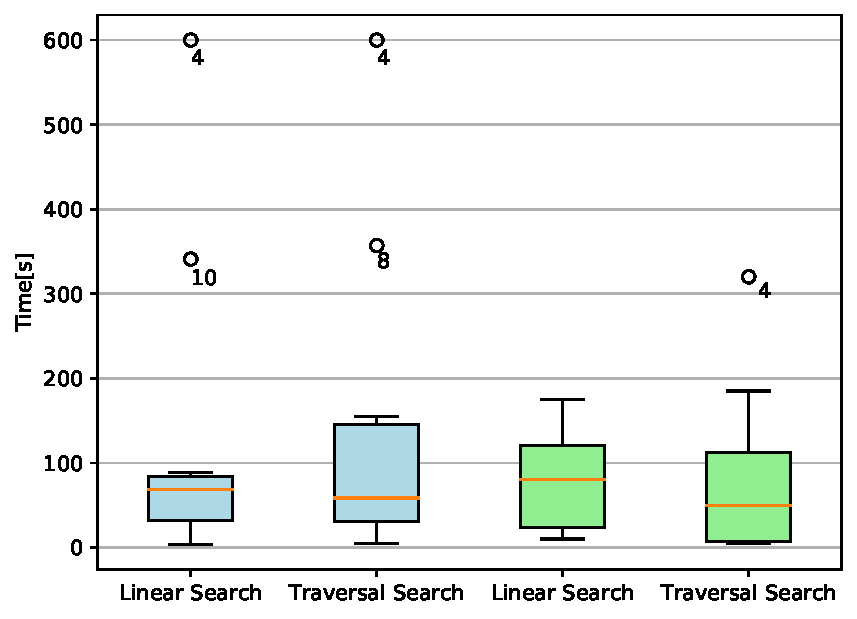
\includegraphics[width=0.7\linewidth]{graphs/face_search_time.pdf}
    \caption[Comparison of the time required to find a target image]{Comparison of the time required to find a target image. Light blue belongs to the respondent A, light green to respondent B. The outliers are identified by the index of the task.}
    \label{fig:search_time}
\end{figure}
\chapter{User Guide}
\label{ch:user_guide}

In the previous chapters, we developed and evaluated several methods for a known-item-search task. In this chapter, we provide a user guide for our implementation of the aforementioned techniques. This chapter only covers user interaction and does not cover experimenting with new datasets nor the overview of the implementation.

The user can access the application via a web-based interface. Once the webpage is opened, we can see by default a module for search based on the collage (refer to \ref{ch:object_location}). The second module includes face similarity search (chapter \ref{ch:face_search}). We proceed to describe both modules.

\section{Running the application}

The easiest way to run the application is to install Docker\footnote{\url{https://docs.docker.com/desktop/}}. Once the Docker is installed, it is enough to run following commands from the top-level directory, i.e., where \verb+README.md+ is located.

\vspace{0.5cm}

\begin{boxedverbatim}
# ./thesis-grizzly/
$ docker build . -t app
$ docker run -p 8000:8000  \
  -v $PWD/image_representations:\
      /diplomova_praca/static/image_representations \
  -t app
\end{boxedverbatim}

\vspace{0.5cm}

Once the application is running, we can access it via browser at following web address: \url{http://127.0.0.1:8000/}. The first initialization takes longer, the website will load itself once the initialization completes. 

\subsection*{Included dataset}

The provided demo includes a small dataset of images to search on. These images come from Open Image Dataset\footnote{\url{https://opensource.google/projects/open-images-dataset}, CC-by 4.0}. The dataset contains 20\,035 images, for which we computed the region splitting for 2x4 regions. For an approach using the antepenultimate layer, we only provide extracted features for half of the dataset, due to the size limit of attachments. Finally, we extracted 528 faces from the dataset used for the search by collage (with the same settings as described in \autoref{ch:face_search}).

The data, which the model uses is in the directory \verb+image_representation+. In the next chapter, we describe how to work with custom data. It is possible to either replace the existing ones or to create a new directory and update the path in the provided example.

\section{Modules}

Our application is separated into two modules: spatial search and face search. Users can switch between the modules in the top right corner. Now we shortly describe a typical interaction of the user with the system for each module.

\subsection{Search by Collage}

The default module, which opens, is search by collage. On the screen, we can see a canvas for creating the queries and some control elements. On the first load, a target image (the searched scene) is displayed for several seconds over the canvas. During the creation of the collage, we can always access the target image by clicking on the image button (``Display hint''), see \autoref{fig:ui_collage}.

\subsubsection*{Creating a collage}

We can create custom collages on the canvas. To add an image to the canvas, we can either \emph{paste} it, or add it via the URL of the image. To paste an image, it needs to be available in the clipboard. The easiest way to do that for most images is to right-click on the image and select ``Copy image''. We can also recommend a selective screenshot feature, which can speed up the copying of the images and add the possibility of selecting only a part of the image. For Windows 10, it is possible via key combination Shift + Win Key + S. Linux users with KDE may use Spectacle (usually invoked via Print Screen key) or a similar utility.

There is no limitation on the number of images in the collage, although the increased number of images may reduce the performance (as they may give misleading hints), and also it prolongs the computation time needed for the query to be processed.

Once the image is placed in the canvas, we can resize it by grabbing the bottom right corner or move it by dragging. To remove the image from the canvas, click on the \verb+x+ button in the top right corner. To submit the query, click the ``Query'' button. By default, automatic querying is turned on, i.e., after each movement or resizing, the system automatically queries the dataset. This can be turned off, which comes handy if the model with longer inference time is used.

It is possible to switch between the approaches used for feature extraction. The list of available approaches can be accessed by clicking on the three dots, next to the query button.

\subsubsection*{Displayed results}

\begin{figure}
    % \centering
    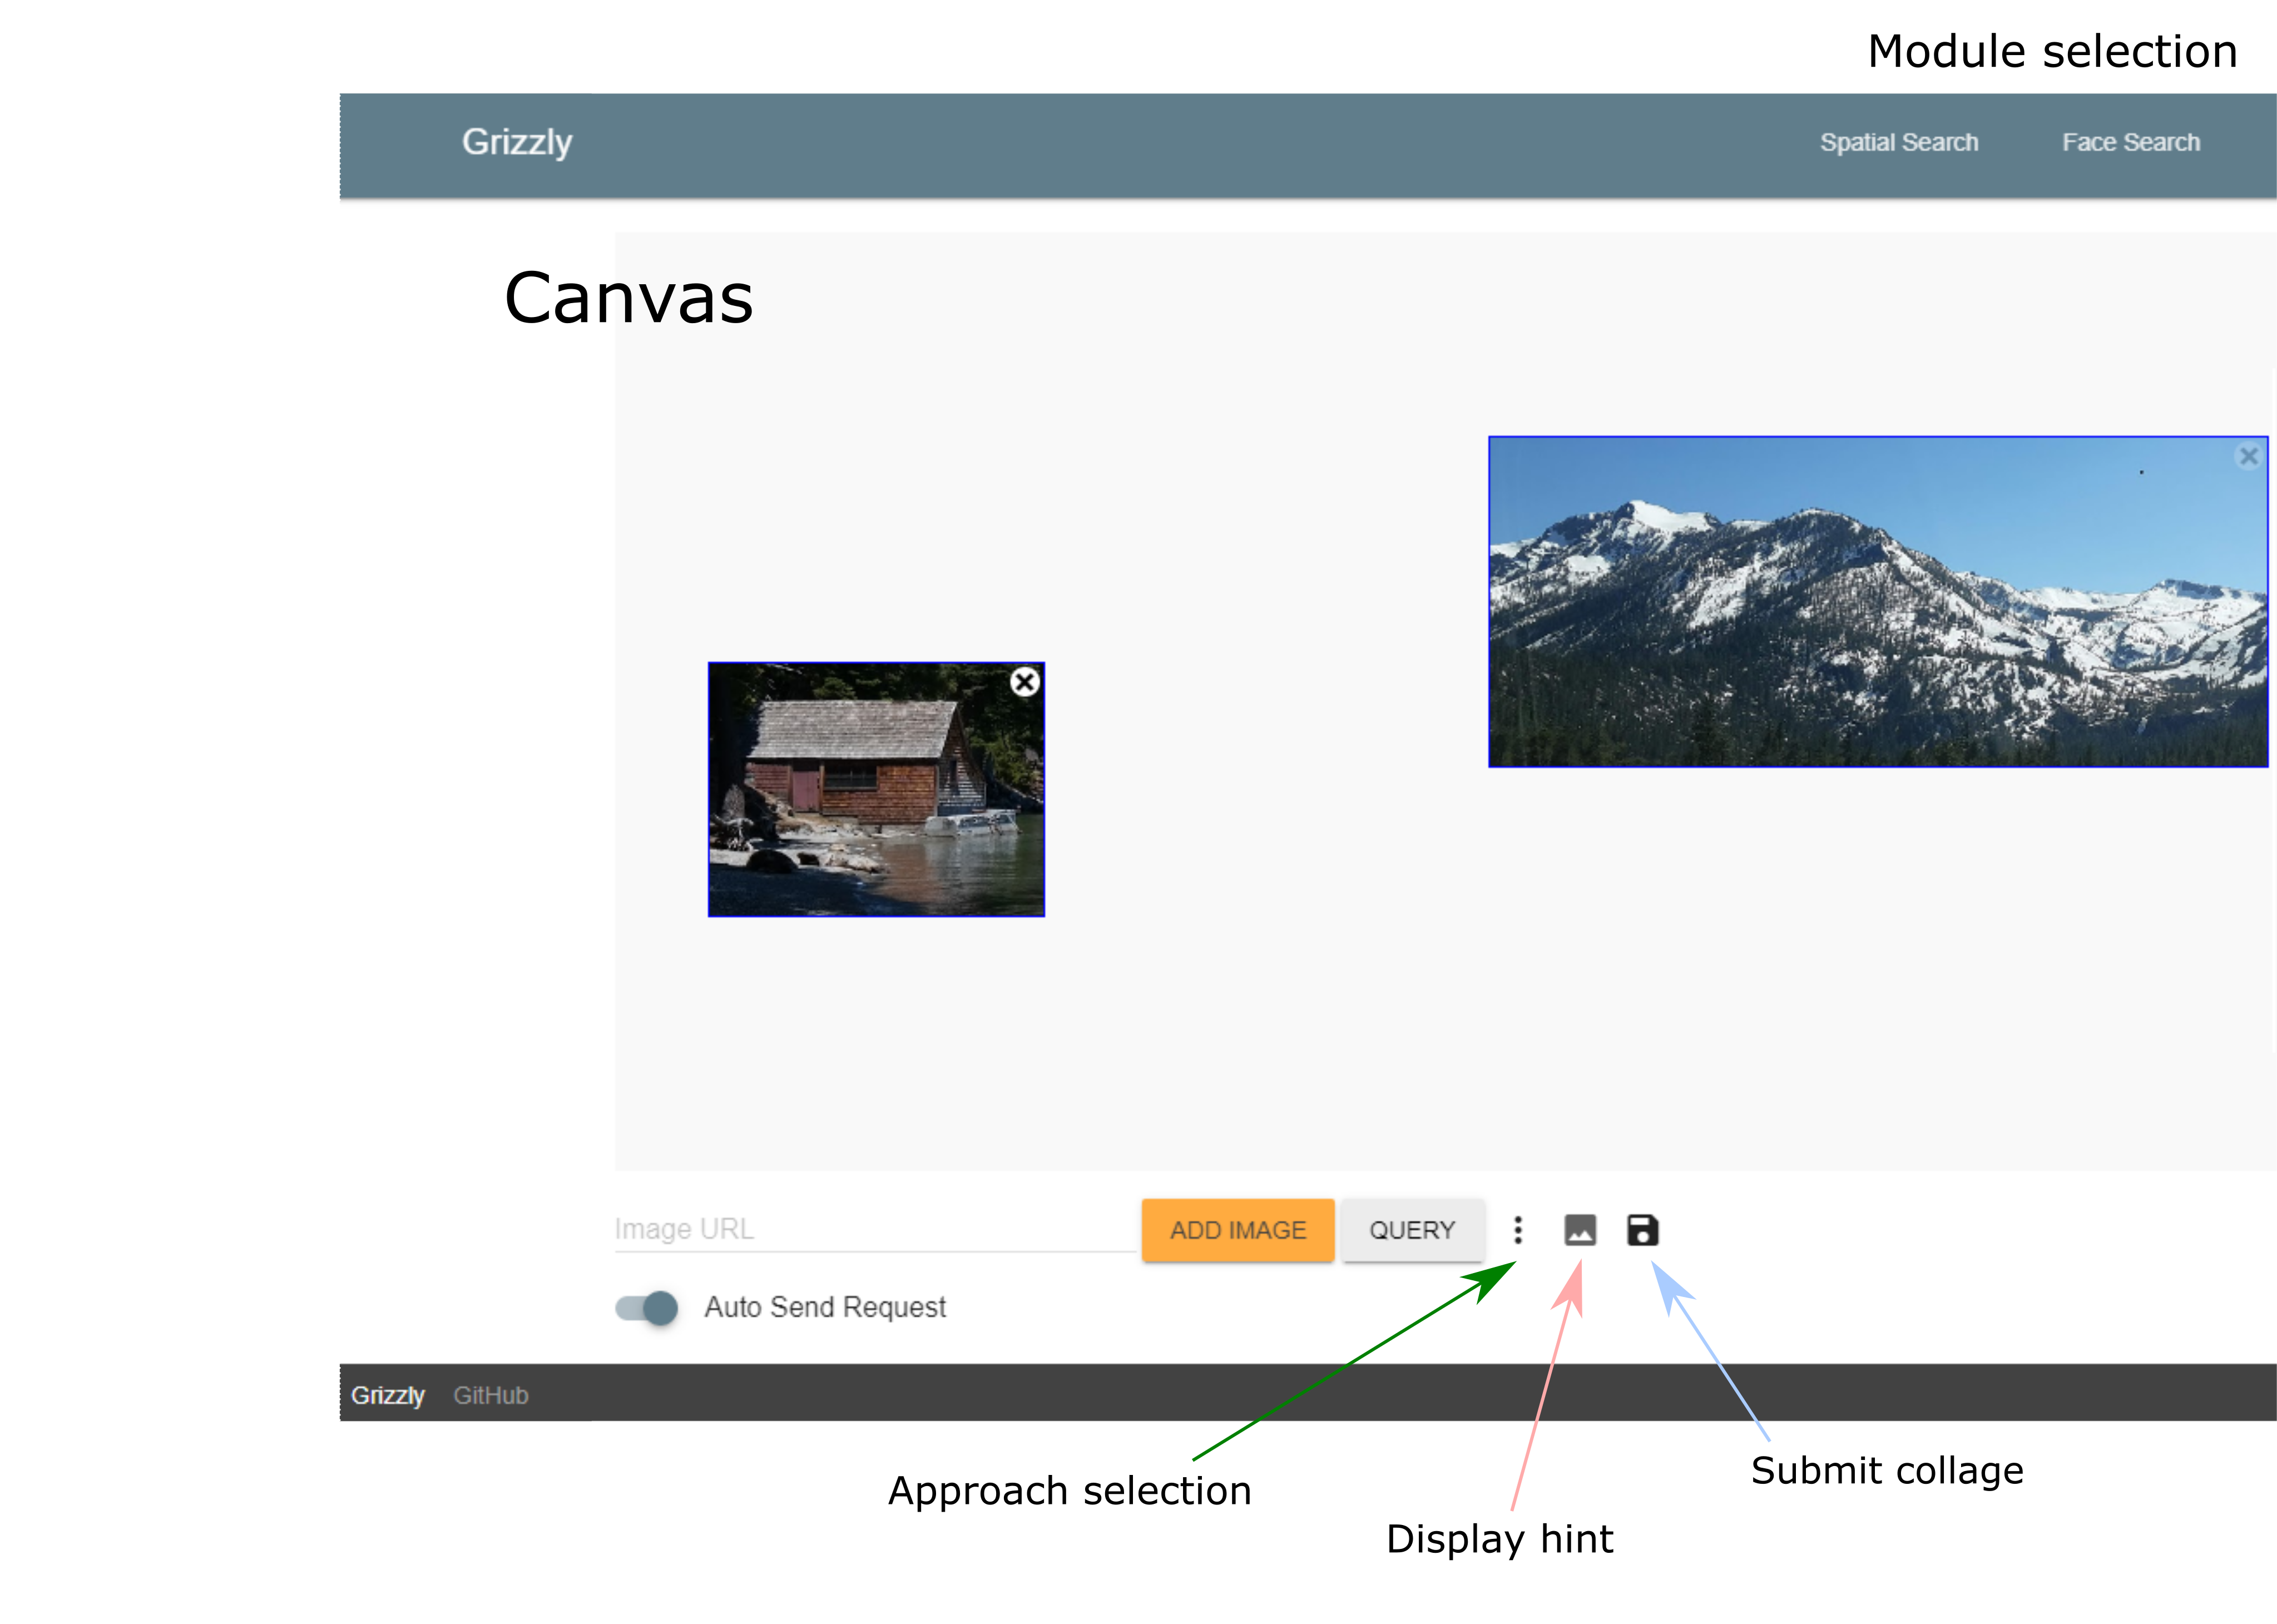
\includegraphics[width=0.9\linewidth]{img/spatial_ui.png}
    \caption{User interface for creating collages}
    \label{fig:ui_collage}
\end{figure}

By default, the application displays only the best 100 matched results. The images are reloaded after each successful query. The top of the Results section also displays the rank of the searched item. This helps the user to learn how to use the tool more effectively. The winning regions are highlighted as well for the regions' search by an orange rectangle.

Results are presented based on the ranking, as we described in \autoref{s:task_formulation}. More similar results are displayed first. If the image is not present in the loaded dataset, the rank will not be displayed. This may be a case if the features for a given approach are not available for all images in the dataset.

\subsection{Search by face similarity}

\begin{figure}
    \centering
    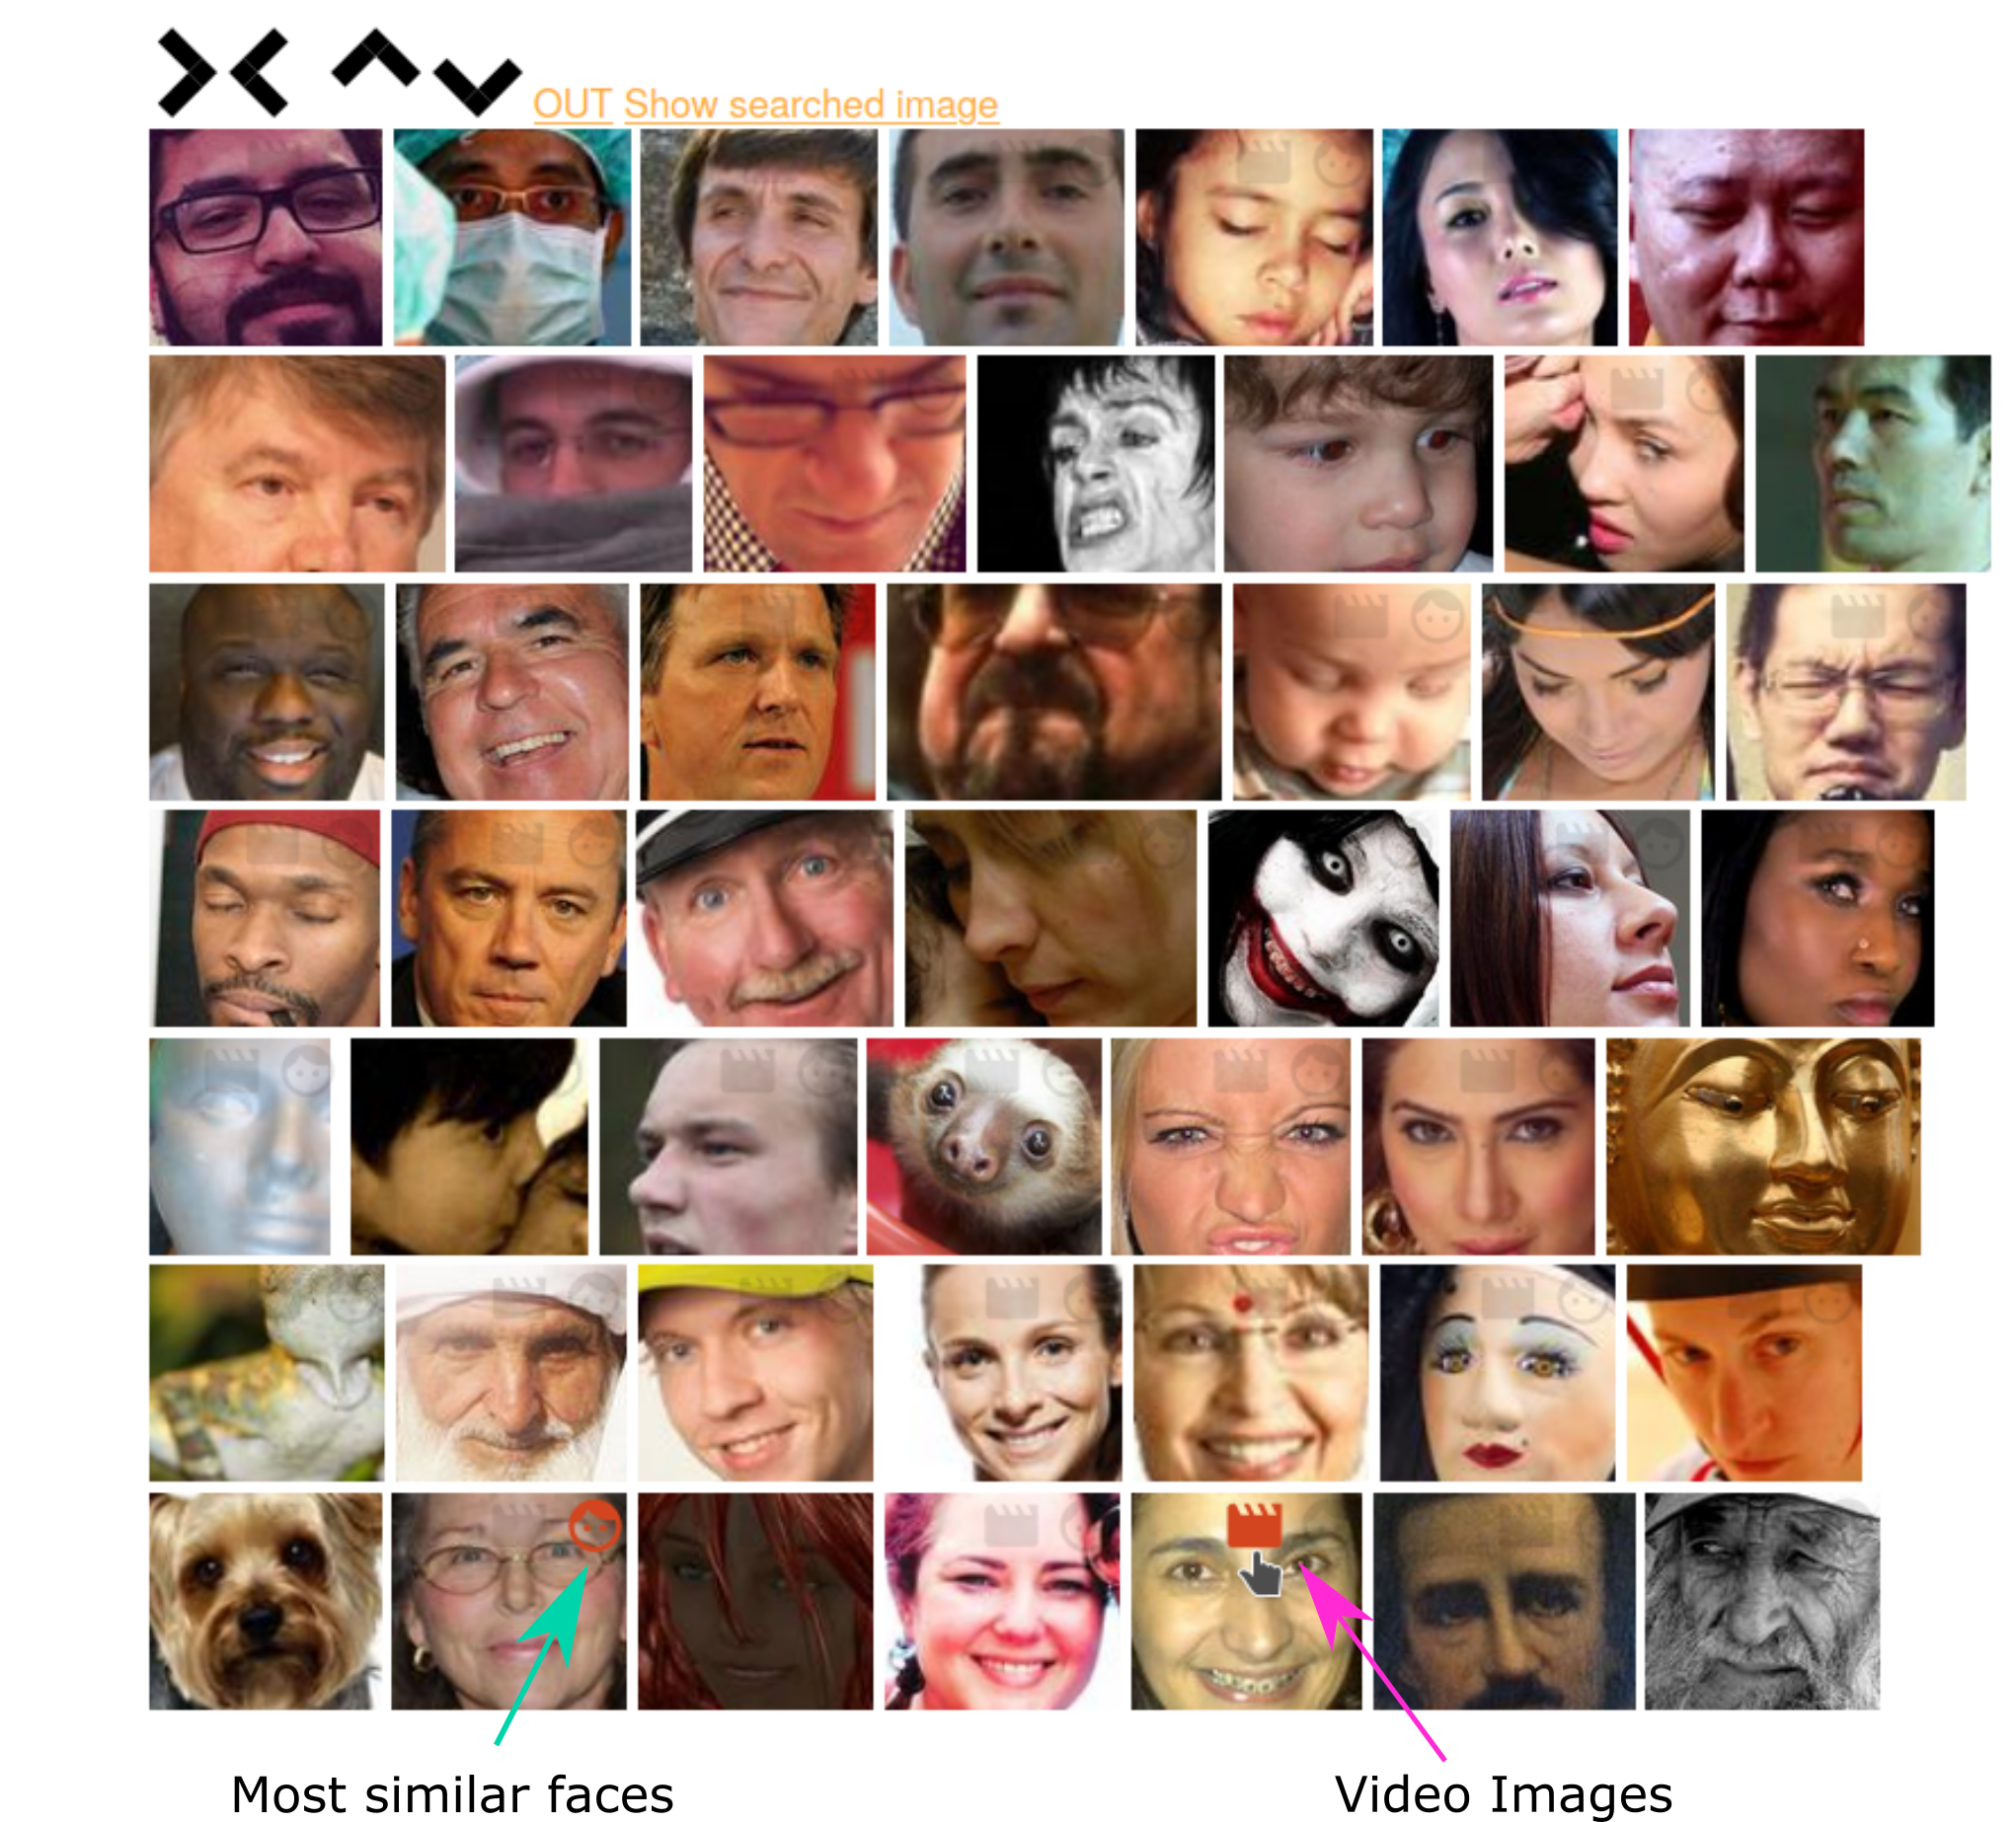
\includegraphics[width=\linewidth]{img/face_grid.png}
    \caption{Top layer of our traversal structure.}
    \label{fig:face_grid_app}
\end{figure}

Upon loading the face module, there is a grid with faces, and also a target image is displayed. Like the Search by collage module, the target image can be accessed at any moment by clicking on \verb+Show the image+. 

The grid, which is displayed, represents the top layer of the multilevel structure. This layer fully fits into a display; therefore, move commands do not have an effect. We can step up from any (except top layer, where it does not have any effect) layer by clicking on the link \verb+Out+.

By clicking at any face, we step down one layer. The image which we clicked is in the center of the next layer, if possible. This is not possible for images near the corners and edges. In such a case, the grid is displayed in a way that full display is used, and the clicked image is as close to the center as possible.

Each image in the traversal structure also supports two additional operations: show images from the video and show the closest faces. In the case of images, which did not come from the videos (the case of the demo dataset), the images displayed by the first option, are arbitrary. The second option displays all images, which contain a face similar to the queried. Both these options are available by corresponding icons in the top right corner of the face, available at any layer. A top layer for our demo dataset is displayed in the figure \ref{fig:face_grid_app}


\chapter{Extracting features for new datasets}
\label{ch:custom_dataset}

In the previous chapter, we described how to run a demo with a preprocessed dataset of images. In this chapter, we describe the steps required to run the application for a new set of images. If we do not want to change the dataset but only evaluate different approaches (i.e., changing the underlying neural network), it is enough to do only the corresponding step.

Our feature extraction is a two-step process. We again use Docker, to avoid dependency problems. The extraction process belongs to separate module -- \verb+diplomova_praca_lib+. Therefore, we firstly change the working directory, and then we build a single docker container, which we use for all extractions.

\vspace{0.5cm}
\begin{boxedverbatim}
$ cd diplomova_praca_lib
$ docker build . -t lib
\end{boxedverbatim}
\vspace{0.5cm}

The user needs to prepare a directory with images to be processed. If the images come from videos, this directory should be further divided into subdirectories. Each subdirectory should then contain images from one video.

\section{Feature extraction for Collage approaches}

In this section, we provide an example of extracting features for our system for both collage approaches: regions and using the last convolution block. In this example, we extract features by \verb+MobileNetV2+, using regions \verb+2x4+ with the \verb+input_size=96+. The system expects equally sized images.

\vspace{0.5cm}
\begin{boxedverbatim}
$ images="/path/to/images/"
$ intermediate_output="/path/to/intermediate_output/"
$ features="/path/to/features/"

$ docker run \
  -v $images:/images \
  -v $intermediate_output:/feature_records \
  lib \
   python diplomova_praca_lib/annotate_images.py \
    --images_dir=/images --save_location=/feature_records \
    --feature_model=mobilenetv2 --num_regions=2,4 \
    --input_size=96

$ docker run \
  -v $intermediate_output:/feature_records \
  -v $features:/features \
  lib \
    python diplomova_praca_lib/preprocess_data.py \
      --input=/feature_records --output=/features 
      --transform --regions --explained_ratio=128
\end{boxedverbatim}

\vspace{0.5cm}

Parameters options for feature extraction are:
\begin{itemize}
    \item \verb+--feature_model+: \verb+resnet50v2antepenultimate+, \verb+resnet50v2+, \\ \verb+mobilenetv2antepenultimate+, \verb+mobilenetv2+, 
    \item \verb+--input_size+: depends on the model used, check with Keras Applications
    \item \verb+--num_regions+: other values evaluated in this thesis were 2x3, 3x5. Other viable options are allowed.
\end{itemize}

The second step includes preprocessing with optional \acrshort{pca} dimension reduction. The parameters are:
\begin{itemize}
    \item \verb+--empty_pipeline+: no \acrshort{pca} is applied, data are only preprocessed forming structure for the application or
    \item \verb+--explained_ratio+: \acrshort{pca} into given number of components is applied
    \item \verb+--regions+: to specify that the data reflect the regions' structure
\end{itemize}

The content of the \verb+$features+ can be then copied to the corresponding directory (see section \ref{s:dir_structure}) and immediately used, by running the app (see chapter \ref{ch:user_guide}).

\section{Feature extraction for Face Similarity}

For the extraction of faces and their encodings, we use similar steps as in the previous section:

\vspace{0.5cm}
\begin{boxedverbatim}
$ images="/path/to/images/"
$ intermediate_output="/path/to/intermediate_output/"
$ features="/path/to/features/"

$ docker run \
  -v $images:/images \
  -v $intermediate_output:/feature_records \
  lib \
   python diplomova_praca_lib/annotate_images.py \
    --images_dir=/images --save_location=/feature_records \
    --feature_model=faces

$ docker run \
  -v $intermediate_output:/feature_records \
  -v $features:/features \
  lib \
    python diplomova_praca_lib/preprocess_face_data.py \
      --input=/feature_records --output=/features \
      --crop_size=0.08
\end{boxedverbatim}
\vspace{0.5cm}

where the \verb+crop_size+ specifies filtering criteria on the minimum area covered by the face in the image.

\subsection{Training Self-organizing map}

After obtaining the face encodings, we can train the underlying self-organizing map, which we use to obtain a grid of faces for the bottom layer.


\vspace{0.5cm}
\begin{boxedverbatim}
$ face_features="/path/to/face_features/"
$ trained_som="/path/to/trained_som/"

$ docker run \
  -v $face_features:/features \
  -v $trained_som:/output \
  lib \
   python diplomova_praca_lib/train_som.py \
    --input=/features \
    --iterations=200000
\end{boxedverbatim}
\vspace{0.5cm}

For \verb+train_som.py+ additional arguments as \verb+learning_rate+, \verb+sigma+, \verb+distance+ may be explored. The scripts saves all intermediate self-organizing maps and also plots the errors during the training. It is possible to choose any of the stored \acrshort{som}s for the application and observe the differences between them.

\section{Running the server with new data}
\label{s:dir_structure}

We can replace any of the existing data by the new ones, either in their original location \verb+images_representations+, or we can create a new location for the data with following structure:


\vspace{0.5cm}
\begin{boxedverbatim}
image_representations/
    faces/
        features/
            faces.npz
        som/
            som.pickle
    images/
        000/
            image1.jpg
        001/
            image2.jpg
    regions/
        model-mobilenetv2,dir=000.npz
        model-mobilenetv2,dir=001.npz
    spatial/
        model-mobilenetv2antepenultimate,dir=000.npz
        model-mobilenetv2antepenultimate,dir=001.npz
\end{boxedverbatim}
\vspace{0.5cm}

It is not necessary to provide all the data for all the approaches. Only the modules with correctly provided data will work as expected.

% \chapter{Title of the second chapter}

\section{Title of the first subchapter of the second chapter}

\section{Title of the second subchapter of the second chapter}


\chapter*{Conclusion}
\addcontentsline{toc}{chapter}{Conclusion}




%%% Bibliography
\normalem
%%% Bibliography (literature used as a source)
%%%
%%% We employ bibTeX to construct the bibliography. It processes
%%% citations in the text (e.g., the \cite{...} macro) and looks up
%%% relevant entries in the bibliography.bib file.
%%%
%%% The \bibliographystyle command selects, which style will be used
%%% for references from the text. The argument in curly brackets is
%%% the name of the corresponding style file (*.bst). Both styles
%%% mentioned in this template are included in LaTeX distributions.

\bibliographystyle{plainnat}    %% Author (year)
% \bibliographystyle{unsrt}     %% [number]

\renewcommand{\bibname}{Bibliography}

%%% Generate the bibliography. Beware that if you cited no works,
%%% the empty list will be omitted completely.

\bibliography{bibliography}

%%% If case you prefer to write the bibliography manually (without bibTeX),
%%% you can use the following. Please follow the ISO 690 standard and
%%% citation conventions of your field of research.

% \begin{thebibliography}{99}
%
% \bibitem{lamport94}
%   {\sc Lamport,} Leslie.
%   \emph{\LaTeX: A Document Preparation System}.
%   2nd edition.
%   Massachusetts: Addison Wesley, 1994.
%   ISBN 0-201-52983-1.
%
% \end{thebibliography}

\ULforem

%%% Figures used in the thesis (consider if this is needed)
\listoffigures

%%% Tables used in the thesis (consider if this is needed)
%%% In mathematical theses, it could be better to move the list of tables to the beginning of the thesis.
% \listoftables

%%% Abbreviations used in the thesis, if any, including their explanation
%%% In mathematical theses, it could be better to move the list of abbreviations to the beginning of the thesis.

% \printglossary[type=\acronymtype]

\printacronyms
\addcontentsline{toc}{chapter}{Acronyms}

%%% Attachments to the master thesis, if any. Each attachment must be
%%% referred to at least once from the text of the thesis. Attachments
%%% are numbered.
%%%
%%% The printed version should preferably contain attachments, which can be
%%% read (additional tables and charts, supplementary text, examples of
%%% program output, etc.). The electronic version is more suited for attachments
%%% which will likely be used in an electronic form rather than read (program
%%% source code, data files, interactive charts, etc.). Electronic attachments
%%% should be uploaded to SIS and optionally also included in the thesis on a~CD/DVD.
%%% Allowed file formats are specified in provision of the rector no. 72/2017.
\appendix
\chapter{Implementation Overview}
\label{ch:developers_guide}
\label{ch:programmers_guide}

When we were creating our application, we kept in mind to make it as easy as possible for users to use. Therefore, we opt for a web-based interface with which users come in contact daily. From the user point of view, it does not require the installation of any additional application, and it can be used across many operating systems.

Creating a simple, shareable environment for users allows us to collect more annotated data. Compared to the classical applications, which need to be installed on each user's computer, a web-based application needs to be set up just on the server by the researcher. Then users can simply access it by the web address. This way, it may be easier to reach a bigger audience.

We decided to use Python for our back-end as it has a big machine learning community with ever-growing possibilities of open-source projects. As a result of this, we decided to use Django -- easily scalable Python web-framework.

Since our implementation covers a wide range of tasks -- from a web-based front-end to a library able to work with deep learning models, we do not include an exhaustive enumeration of the specific classes and functions in this chapter. Instead, we provide an overview of the individual parts of the application. We start with the separation of the application into three layers, as displayed in figure \ref{fig:implementation_overview}.

This figure represents the individual layers of our solution and provides a summary of the technologies used in the layers. Our application consists of two main Python modules: \verb+diplomova_praca+ and \verb+diplomova_praca_lib+. In the figure, the front-end and back-end belong to the first one, and the library represents module \verb+diplomova_praca_lib+.

We shortly describe each of the parts, as displayed in the figure.

\section{Front-end}

Our front-end consists of several Django templates (a way to create HTML files dynamically), with the corresponding styling. We then use jQuery to provide a user with an interactive environment in the application.  The part of displaying the menu and the results are shared between both modules -- face and spatial. The interactive content -- canvas for the spatial and the grid for faces -- is dynamically added based on the currently selected module.

\subsubsection*{Design}
For a unified look, we follow the Material Design guidelines. We use some of the components from Material Design Lite. To complement the overall design, we also use Material Design Icons.

We use the Material Design components with our own elements using the Cascading Style Sheets. We use Syntactically Awesome Style Sheets (commonly known as SCSS) to reduce the amount of code. One of the advantages of SCSS compared to CSS is the support of variables and nesting. We use this, for example, when setting the colors for the whole application. This way, we can provide users with a unified color scheme, while the colors can be easily adjusted for a different color scheme.

\subsubsection*{Interaction}

To provide a smooth user experience, without any unnecessary loading during the search, we use JavaScript. For some actions, like dragging, resizing we utilize functionalities from jQuery\footnote{\url{https://jquery.com/}}. 

To avoid reloadings, we update the content using JavaScript and obtain the data via asynchronous communication with our Django back-end. One of the advantages of this approach is that the user can continue to experiment with the collage while the system is retrieving the results.

We do the communication with the Django as asynchronous HTTP POST requests. We encode the data as JSON, or directly as a string, if possible. The data are of different types; for example, in the spatial module, we need to send all images with their relative position. In the case of the face module, we include the Tree View, i.e., the current level and position in the layer.

\section{Back-end}

The goal of our back-end is to process the HTTP requests from front-end and transform them into Python objects. This way, we can directly query our library by calling the functions by passing the Python objects. The back-end also initializes the datasets in the library. Additional functionality of the back-end is the choice of the target image out of available images. Secondary functionalities include logging submitted collages and additional data into the database.

\section{Library}

In the library, we implement all approaches mentioned in this thesis. The library includes all the feature extraction methods, image handling, training, plots generation, and more.

Since the content of the library is broad, we could separate it further into four main blocks: 
\begin{itemize}
    \item Annotation and Preprocessing -- scripts used for extraction of the features from a custom dataset
    \item \verb+face_features/+ -- face module, which is responsible for creating the multilevel structure (\verb+TreeView+). It also contains models for the extraction of faces and the feature extraction.
    \item \verb+position_similarity/+ -- spatial module, which includes used models and the feature extraction techniques (as regions or antepenultime approach). The entry point for any request is \verb+positional_request()+ in \verb+position_similarity_request.py+. We use this entry point for our experiments.
    \item Additional scripts (\verb+helpers/+) -- this includes all the scripts to run and evaluate the experiments.. These are not necessary for the application itself, but useful while investigating the approaches.
\end{itemize}

\subsubsection*{Attribution}

At last, we would like to express our gratitude to the authors of all the used technologies provided by an open-source community. Additionally, to the projects mentioned in the text, we would like to thank the authors of crucial libraries such as Scikit-learn \citep{pedregosa2011scikit} and NumPy \citep{van2011numpy}.

\begin{figure}
    \centering
    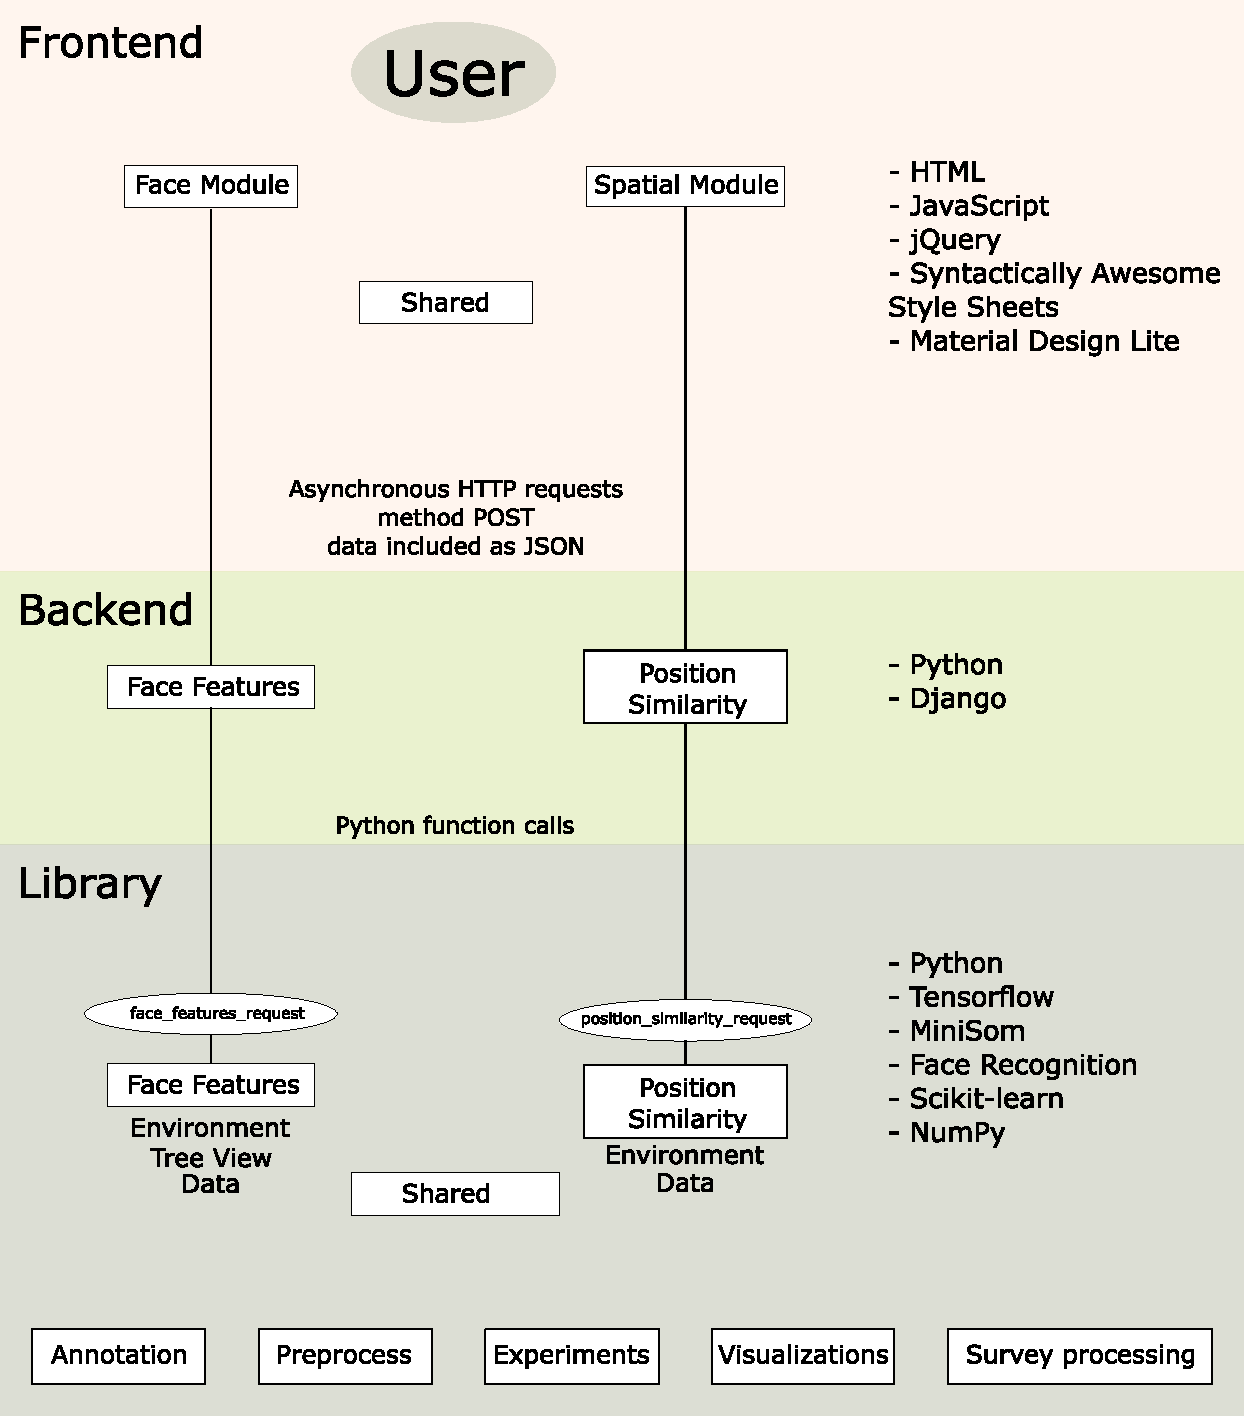
\includegraphics[width=0.95\linewidth]{graphs/implementation_overview.pdf}
    \caption{Overview of the implementation}
    \label{fig:implementation_overview}
\end{figure}
% \chapter{Attachments}

% \section{First Attachment}

\openright
\end{document}
